

\chapter{Release 3:Gestion des Offres d'Emploi,Projets Freelance,et Système de Messagerie }

\DeclareRobustCommand{\greencheck}{%
  \tikz\fill[scale=0.4, color=green]
  (0,.35) -- (.25,0) -- (1,.7) -- (.25,.15) -- cycle;%
}

\minitoc
\newpage
\section*{Introduction}
\addcontentsline{toc}{section}{Introduction}
Dans le cadre de la cinquième phase du développement de notre application, nous avons concentré nos efforts sur trois modules essentiels : la gestion des offres d'emploi, les projets freelance et le système de messagerie. Ces fonctionnalités constituent une extension significative de notre plateforme, permettant aux utilisateurs de trouver des opportunités professionnelles, de proposer ou postuler à des projets freelance, et de communiquer efficacement entre eux.

\section{Objectifs du Sprint 5}

\subsection{Gestion des Offres d'Emploi}
L'objectif de ce module est de permettre aux entreprises de publier des offres d'emploi détaillées, incluant une géolocalisation, et aux utilisateurs de rechercher et postuler à ces offres selon différents critères. Les entreprises pourront également gérer les candidatures reçues en suivant leur statut, tandis que les candidats seront notifiés des évolutions de leurs candidatures. Ce module vise à créer un écosystème complet pour la recherche d'emploi, facilitant la mise en relation entre entreprises et candidats.

\subsection{Projets Freelance}
Ce module a pour but de créer un espace où les utilisateurs peuvent publier des projets freelance avec des spécifications précises, et où les freelances peuvent soumettre des propositions détaillées. Le système permet la gestion complète du cycle de vie d'un projet, depuis sa publication jusqu'à la contractualisation, en passant par l'évaluation des propositions. La mise en place de jalons et la signature électronique des contrats assurent une collaboration structurée et sécurisée entre les parties.

\subsection{Système de Messagerie}
L'objectif de ce module est d'implémenter un système de communication complet au sein de la plateforme, permettant aux utilisateurs d'échanger des messages directs, de créer des conversations de groupe, et de partager différents types de médias. Les fonctionnalités de notification, de recherche dans l'historique et de gestion des statuts de lecture visent à offrir une expérience de communication fluide et efficace, essentielle pour la collaboration professionnelle.

\section{Backlog Fonctionnel —“ Sprint 5}

\subsection{Backlog Produit —“ Offres d'Emploi}
Le tableau ci-dessous recense les user stories associées à la gestion des offres d'emploi. 

\usepackage{tabularx}
\usepackage{float}
\usepackage{caption}

\begin{table}[H]
\centering
\begin{tabularx}{\textwidth}{|c|X|c|}
\hline
\textbf{User Story} & \textbf{Description} & \textbf{Priorité} \\
\hline
US-01 & En tant qu'entreprise, je veux pouvoir publier des offres d'emploi avec titre, description, compétences requises, type de contrat et localisation. & Haute \\
\hline
US-02 & En tant qu'entreprise, je veux pouvoir géolocaliser mes offres d'emploi. & Moyenne \\
\hline
US-03 & En tant qu'utilisateur, je veux pouvoir rechercher des offres d'emploi par localisation avec un rayon de distance. & Haute \\
\hline
US-04 & En tant qu'utilisateur, je veux pouvoir filtrer les offres d'emploi par domaine, type de contrat et niveau d'expérience. & Haute \\
\hline
US-05 & En tant qu'utilisateur, je veux pouvoir postuler aux offres d'emploi avec mon CV et lettre de motivation. & Haute \\
\hline
US-06 & En tant qu'entreprise, je veux pouvoir consulter toutes les candidatures reçues pour mes offres. & Haute \\
\hline
US-07 & En tant qu'entreprise, je veux pouvoir gérer le statut des candidatures (nouvelle, en cours, acceptée, rejetée). & Moyenne \\
\hline
\end{tabularx}
\end{table}
\begin{table}[H]
\centering
\begin{tabularx}{\textwidth}{|c|X|c|}
\hline
\textbf{User Story} & \textbf{Description} & \textbf{Priorité} \\
\hline
US-08 & En tant qu'utilisateur, je veux être notifié du changement de statut de mes candidatures. & Moyenne \\
\hline
US-09 & En tant qu'entreprise, je veux pouvoir activer/désactiver mes offres d'emploi. & Moyenne \\
\hline
US-10 & En tant qu'entreprise, je veux pouvoir générer automatiquement un contrat d'embauche lorsque j'accepte une candidature. & Haute \\
\hline
US-11 & En tant qu'utilisateur, je veux pouvoir consulter, accepter et signer électroniquement un contrat d'embauche. & Haute \\
\hline
US-12 & En tant qu'entreprise, je veux recevoir une notification lorsqu'un candidat signe un contrat d'embauche. & Moyenne \\
\hline
\end{tabularx}
\caption{User Stories liées aux offres d'emploi}
\end{table}



\subsection{Backlog Produit —“ Projets Freelance}
Le tableau ci-dessous présente les user stories liées à la gestion des projets freelance, permettant aux employeurs de publier des projets et aux freelances de proposer leurs services.

\begin{table}[H]
\centering
\begin{tabularx}{\textwidth}{|c|X|c|}
\hline
\textbf{User Story} & \textbf{Description} & \textbf{Priorité} \\
\hline
US-13 & En tant qu'employeur, je veux pouvoir publier des projets avec titre, description, budget, durée, compétences requises et catégorie. & Haute \\
\hline
US-14 & En tant qu'employeur, je veux pouvoir joindre des documents à mes projets. & Moyenne \\
\hline
US-15 & En tant que freelance, je veux pouvoir parcourir les projets disponibles avec filtres (catégorie, budget, compétences). & Haute \\
\hline
US-16 & En tant que freelance, je veux pouvoir soumettre des propositions pour des projets avec lettre de motivation, prix proposé et durée estimée. & Haute \\
\hline
US-17 & En tant que freelance, je veux pouvoir définir des jalons (milestones) précis pour mes propositions de projets. & Moyenne \\
\hline
US-18 & En tant que freelance, je veux pouvoir joindre des documents à mes propositions. & Moyenne \\
\hline
US-19 & En tant qu'employeur, je veux pouvoir consulter toutes les propositions reçues pour mes projets. & Haute \\
\hline
US-20 & En tant qu'employeur, je veux pouvoir accepter une proposition et générer automatiquement un contrat. & Haute \\
\hline
\end{tabularx}
\end{table}
\begin{table}[H]
\centering
\begin{tabularx}{\textwidth}{|c|X|c|}
\hline
\textbf{User Story} & \textbf{Description} & \textbf{Priorité} \\
\hline
US-21 & En tant qu'utilisateur (employeur ou freelance), je veux pouvoir signer un contrat électroniquement. & Haute \\
\hline
US-22 & En tant qu'utilisateur, je veux recevoir des notifications concernant les mises à jour de statut des projets. & Moyenne \\
\hline
US-23 & En tant qu'utilisateur, je veux pouvoir consulter les statistiques sur mes projets. & Basse \\
\hline
US-24 & En tant qu'employeur, je veux pouvoir personnaliser certaines clauses du contrat avant sa génération. & Moyenne \\
\hline
US-25 & En tant qu'utilisateur, je veux pouvoir consulter l'historique de tous mes contrats (en cours et terminés). & Moyenne \\
\hline
US-26 & En tant qu'utilisateur, je veux pouvoir télécharger une copie de mes contrats signés en format PDF sécurisé. & Haute \\
\hline
US-27 & En tant qu'utilisateur, je veux recevoir des notifications pour les échéances contractuelles liées aux jalons du projet. & Moyenne \\
\hline
US-28 & En tant qu'utilisateur, je veux pouvoir proposer des avenants au contrat initial en cas de modification du périmètre du projet. & Moyenne \\
\hline
\end{tabularx}
\caption{User Stories liées aux projets freelance}
\end{table}


\subsection{Backlog Produit —“ Messagerie}
Ce tableau présente les user stories associées au système de messagerie, permettant aux utilisateurs de communiquer efficacement sur la plateforme.

\begin{table}[H]
\centering
\begin{tabularx}{\textwidth}{|c|X|c|}
\hline
\textbf{User Story} & \textbf{Description} & \textbf{Priorité} \\
\hline
US-29 & En tant qu'utilisateur, je veux pouvoir envoyer des messages directs à d'autres utilisateurs. & Haute \\
\hline
US-30 & En tant qu'utilisateur, je veux pouvoir créer des conversations de groupe avec plusieurs participants. & Moyenne \\
\hline
US-31 & En tant qu'utilisateur, je veux pouvoir partager des images, fichiers et autres médias dans mes messages. & Moyenne \\
\hline
US-32 & En tant qu'utilisateur, je veux recevoir des notifications pour les nouveaux messages. & Haute \\
\hline
US-33 & En tant qu'utilisateur, je veux pouvoir rechercher dans l'historique de mes conversations. & Basse \\
\hline
US-34 & En tant qu'utilisateur, je veux voir le statut de lecture de mes messages (lu/non lu). & Basse \\
\hline
US-35 & En tant qu'utilisateur, je veux pouvoir ajouter ou retirer des membres d'une conversation de groupe. & Moyenne \\
\hline
US-36 & En tant qu'utilisateur, je veux pouvoir quitter une conversation de groupe. & Basse \\
\hline
\end{tabularx}
\caption{User Stories liées à la messagerie}
\end{table}

\section{Raffinement des cas d'utilisation}
\subsection{Raffinement des cas d'utilisation - Offres d'emploi}
\subsubsection{Raffinement du cas d'utilisation "Gestion des offres d'emploi"}
La figure 5.1 présente le raffinement du cas d'utilisation "Publier une offre d'emploi", suivie par sa description textuelle dans le tableau 5.4.

% Insérer ici l'image du diagramme de cas d'utilisation
\begin{figure}[H]
    \centering
    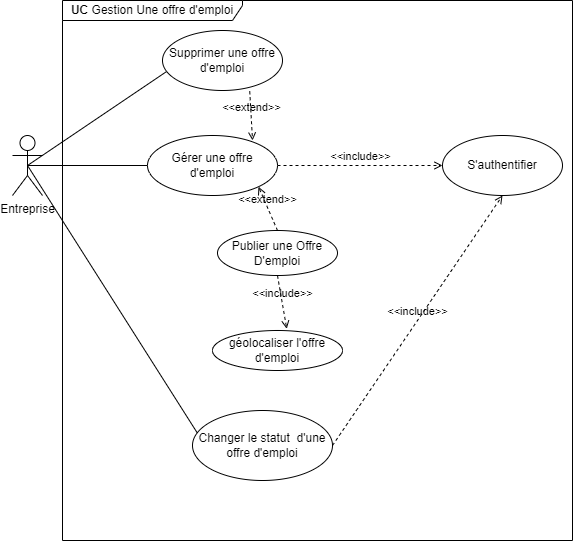
\includegraphics[width=0.8\textwidth]{images/publierOffreEmploifinale1.drawio.png}
    \caption{Diagramme des cas d'utilisation Publier une offre d'emploi}
    \label{fig:publier_offre_emploi}
\end{figure}
\begin{table}[H]
\centering
\begin{tabular}{|p{4cm}|p{10cm}|}
\hline
\textbf{Élément} & \textbf{Description} \\ \hline
Cas d'utilisation & Publier une offre d'emploi \\ \hline
Acteur & Entreprise \\ \hline
Précondition & L'entreprise est authentifiée dans le système. \\ \hline
Postcondition & L'offre d'emploi est publiée et visible pour les utilisateurs. \\ \hline
Scénario nominal & 
1. L'entreprise s'authentifie. \newline
2. L'entreprise accède à la section de gestion des offres d'emploi. \newline
3. L'entreprise sélectionne "Créer une nouvelle offre". \newline
4. L'entreprise remplit les champs requis (titre, description, compétences, type de contrat, localisation). \newline
5. L'entreprise peut ajouter une géolocalisation précise. \newline
6. L'entreprise soumet le formulaire. \newline
7. Le système valide les informations et publie l'offre. \newline
8. L'entreprise reçoit une confirmation de publication. \\ \hline
Scénario alternatif & 
4a. Si des champs obligatoires sont incomplets, le système affiche un message d'erreur et invite à compléter les informations manquantes. \newline
6a. Si la validation échoue, l'entreprise est informée des erreurs à corriger. \\ \hline
\end{tabular}
\caption{Description textuelle du cas d'utilisation Publier une offre d'emploi}
\end{table}

\subsubsection{Raffinement du cas d'utilisation "Postuler à une offre d'emploi"}
La figure 5.2 présente le raffinement du cas d'utilisation "Postuler à une offre d'emploi", suivie par sa description textuelle dans le tableau 5.5.

% Insérer ici l'image du diagramme de cas d'utilisation
\begin{figure}[H]
    \centering
    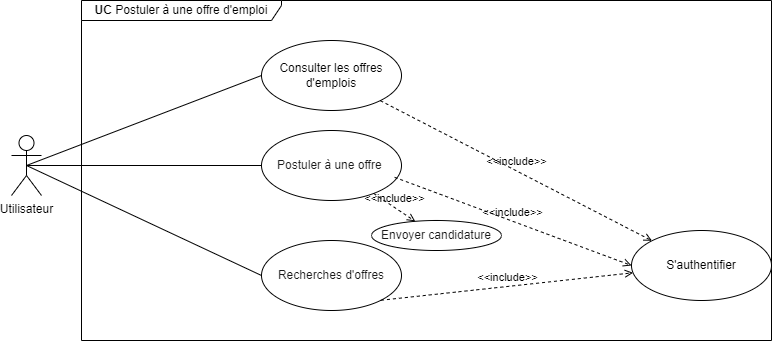
\includegraphics[width=0.8\textwidth]{images/Postuleruneoffred'emploifinale.drawio.png}
    \caption{Diagramme des cas d'utilisation Postuler à une offre d'emploi}
    \label{fig:postuler_offre_emploi}
\end{figure}
Lors de la recherche d'offres d'emploi sur notre plateforme, l'utilisateur a la possibilité d'affiner ses résultats grâce à plusieurs filtres. Il peut notamment spécifier le niveau d'expérience requis, le domaine d'activité, le type de contrat (CDI, CDD, stage, etc.), ainsi que la localisation géographique à l'aide d'une carte interactive. Ces filtres permettent de cibler rapidement les opportunités correspondant au profil et aux préférences du candidat, rendant la recherche plus efficace et personnalisée.
\begin{table}[H]
\centering
\begin{tabular}{|p{4cm}|p{10cm}|}
\hline
\textbf{Élément} & \textbf{Description} \\ \hline
Cas d'utilisation & Postuler à une offre d'emploi \\ \hline
Acteur & Utilisateur \\ \hline
Précondition & L'utilisateur est authentifié et l'offre d'emploi est active. \\ \hline
Postcondition & La candidature est soumise et visible par l'entreprise. \\ \hline
Scénario nominal & 
1. L'utilisateur s'authentifie. \newline
2. L'utilisateur recherche et filtre les offres d'emploi. \newline
3. L'utilisateur consulte les détails d'une offre qui l'intéresse. \newline
4. L'utilisateur sélectionne "Postuler". \newline
5. L'utilisateur soumet son CV et sa lettre de motivation. \newline
6. Le système enregistre la candidature. \newline
7. L'utilisateur reçoit une confirmation de soumission. \newline
8. L'entreprise est notifiée de la nouvelle candidature. \\ \hline
Scénario alternatif & 
5a. Si l'utilisateur a déjà postulé à cette offre, le système affiche un message l'informant de sa candidature existante. \newline
5b. Si des documents requis sont manquants, le système invite l'utilisateur à les fournir. \\ \hline
\end{tabular}
\caption{Description textuelle du cas d'utilisation Postuler à une offre d'emploi}
\end{table}

\subsection{Raffinement des cas d'utilisation - Projets Freelance}

\subsubsection{Raffinement du cas d'utilisation "Soumettre une proposition pour un projet"}
La figure 5.3 présente le raffinement du cas d'utilisation "Soumettre une proposition pour un projet", suivie par sa description textuelle dans le tableau 5.6.

% Insérer ici l'image du diagramme de cas d'utilisation
\begin{figure}[H]
    \centering
    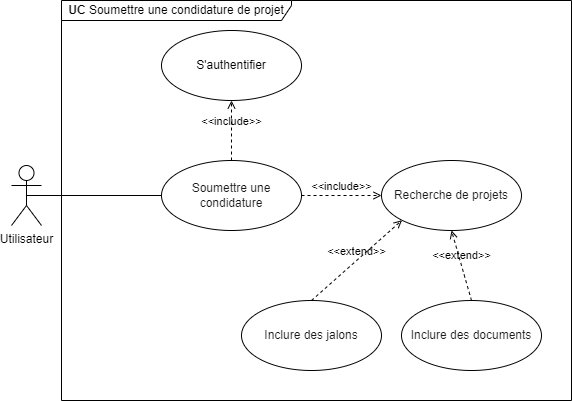
\includegraphics[width=0.8\textwidth]{images/SoumettreunePropositionfinale1.drawio.png}
    \caption{Diagramme des cas d'utilisation Soumettre une proposition pour un projet}
    \label{fig:soumettre_prop_projet_freelance}
\end{figure}
\begin{table}[H]
\centering
\begin{tabular}{|p{4cm}|p{10cm}|}
\hline
\textbf{Élément}        & \textbf{Description} \\ \hline
Cas d'utilisation       & Soumettre une proposition pour un projet \\ \hline
Acteur                  &utilisateur\\ \hline
Précondition            & L'utilisateur est authentifié et le projet est actif. \\ \hline
Postcondition           & La proposition est soumise et visible par l'employeur(utilisateur). \\ \hline
\end{tabular}

\end{table}

\begin{table}[H]
\centering
\begin{tabular}{|p{4cm}|p{10cm}|}
\hline

Scénario nominal        & 
1. L'utilisateur s'authentifie. \newline
2. IL parcourt et filtre les projets disponibles. \newline
3. IL consulte les détails d'un projet qui l'intéresse. \newline
4. IL sélectionne "Soumettre une proposition". \newline
5. IL rédige sa lettre de motivation, indique son prix proposé et sa durée estimée. \newline
6. IL peut définir des jalons (milestones) pour la réalisation. \newline
7. IL peut joindre des documents à sa proposition. \newline
8. IL soumet sa proposition. \newline
9. Le système enregistre la proposition. \newline
10. IL reçoit une confirmation de soumission. \newline
11. L'employeur est notifié de la nouvelle proposition. \\ \hline
Scénario alternatif     & 
5a. Si le freelance a déjà soumis une proposition pour ce projet, le système l'informe de sa proposition existante et lui propose de la modifier. \newline
7a. Si la taille des documents dépasse la limite autorisée, le système informe le freelance et demande de réduire la taille ou de changer les fichiers. \\ \hline
\end{tabular}
\caption{Description textuelle du cas d'utilisation Soumettre une proposition pour un projet}
\end{table}


\subsubsection{Raffinement du cas d'utilisation "Gérer les contrats"}
La figure 5.4 présente le raffinement du cas d'utilisation "Gérer les contrats", suivie par sa description textuelle dans le tableau 5.7.

% Insérer ici l'image du diagramme de cas d'utilisation
\begin{figure}[H]
    \centering
    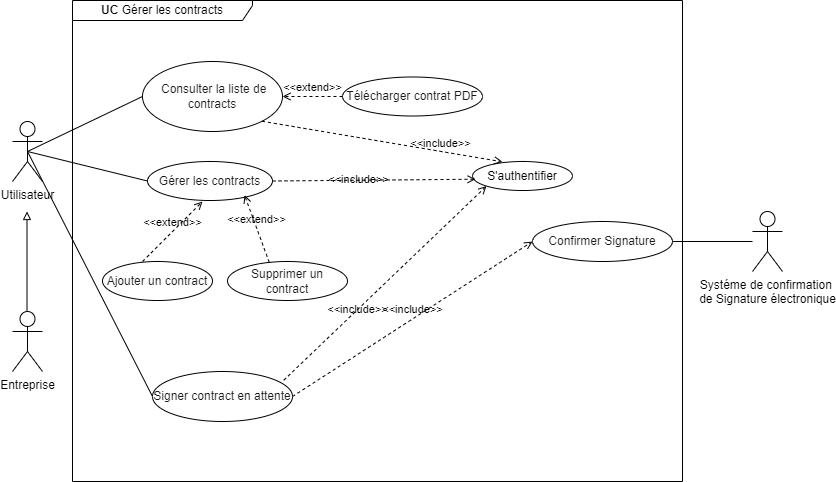
\includegraphics[width=0.8\textwidth]{images/GérerContractUcfinale1.drawio.png}
    \caption{Diagramme des cas d'utilisation Gérer les contrats}
    \label{fig:gerer_contrats}
\end{figure}
\begin{table}[H]
\centering
\begin{tabular}{|p{4cm}|p{10cm}|}
\hline
\textbf{Élément} & \textbf{Description} \\ \hline
Cas d'utilisation & Gérer les contrats \\ \hline
Acteurs & Employeur, Freelance \\ \hline
Précondition & L'utilisateur est authentifié dans le système et a au moins un contrat en cours ou terminé. \\ \hline
Postcondition & Les actions sur les contrats sont exécutées et enregistrées. \\ \hline
Scénario nominal & 
1. L'utilisateur s'authentifie. \newline
2. L'utilisateur accède à la section de gestion des contrats. \newline
3. L'utilisateur peut : \newline
\hspace{0.5cm} a. Consulter la liste de ses contrats. \newline
\hspace{0.5cm} b. Visualiser les détails d'un contrat spécifique. \newline
\hspace{0.5cm} c. Signer électroniquement un contrat en attente. \newline
\hspace{0.5cm} d. Télécharger une copie du contrat en PDF. \newline
\hspace{0.5cm} e. Proposer un avenant à un contrat existant. \newline
\hspace{0.5cm} f. Suivre les jalons contractuels. \newline
4. Le système exécute l'action demandée. \newline
5. L'utilisateur reçoit une confirmation de l'action effectuée. \\ \hline
Scénario alternatif & 
3c. Si l'utilisateur a déjà signé le contrat, le système l'en informe. \newline
3e. Si le contrat ne permet pas d'avenant, le système affiche un message explicatif. \newline
3f. Si aucun jalon n'est défini, le système affiche un message approprié. \\ \hline
\end{tabular}
\caption{Description textuelle du cas d'utilisation Gérer les contrats}
\end{table}

\subsection{Raffinement des cas d'utilisation - Messagerie}
\subsubsection{Raffinement du cas d'utilisation "Envoyer un message direct"}
La figure 5.5 présente le raffinement du cas d'utilisation "Envoyer un message direct", suivie par sa description textuelle dans le tableau 5.8.

% Insérer ici l'image du diagramme de cas d'utilisation
\begin{figure}[H]
    \centering
    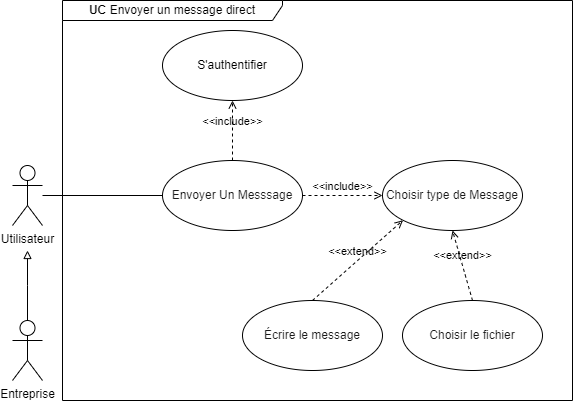
\includegraphics[width=0.8\textwidth]{images/EnvoyerunMessagefinale.drawio.png}
    \caption{Diagramme des cas d'utilisation Envoyer un message direct}
    \label{fig:Envoie_message_direct}
\end{figure}
\begin{table}[H]
\centering
\begin{tabular}{|p{4cm}|p{10cm}|}
\hline
\textbf{Élément} & \textbf{Description} \\ \hline
Cas d'utilisation & Envoyer un message direct \\ \hline
Acteur & Utilisateur \\ \hline
Précondition & L'utilisateur est authentifié dans le système. \\ \hline
Postcondition & Le message est envoyé et visible par le destinataire. \\ \hline
Scénario nominal & 
1. L'utilisateur s'authentifie. \newline
2. L'utilisateur accède à la messagerie. \newline
3. L'utilisateur sélectionne un contact existant ou cherche un nouvel utilisateur. \newline
4. L'utilisateur ouvre la conversation. \newline
5. L'utilisateur rédige son message. \newline
6. L'utilisateur peut joindre des médias (images, fichiers). \newline
7. L'utilisateur envoie le message. \newline
8. Le système transmet le message. \newline
9. Le destinataire reçoit une notification. \\ \hline
Scénario alternatif & 
3a. Si l'utilisateur recherché n'existe pas, le système affiche un message approprié. \newline
6a. Si la taille des médias dépasse la limite autorisée, le système informe l'utilisateur et demande de réduire la taille ou de changer les fichiers. \newline
8a. Si la connexion est perdue, le message est mis en attente d'envoi. \\ \hline
\end{tabular}
\caption{Description textuelle du cas d'utilisation Envoyer un message direct}
\end{table}

\subsubsection{Raffinement du cas d'utilisation "Créer une conversation de groupe"}
La figure 5.6 présente le raffinement du cas d'utilisation "Créer une conversation de groupe", suivie par sa description textuelle dans le tableau 5.9.

% Insérer ici l'image du diagramme de cas d'utilisation
\begin{figure}[H]
    \centering
    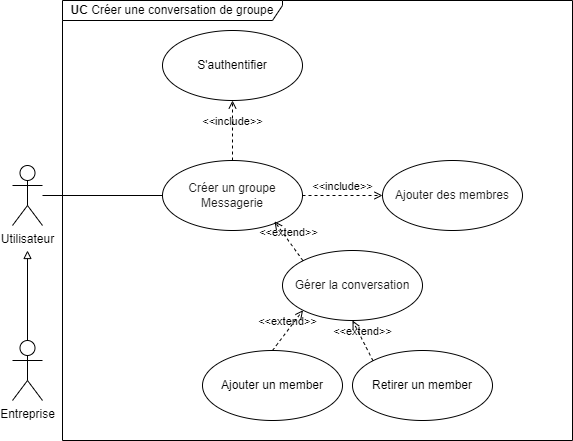
\includegraphics[width=0.8\textwidth]{images/Créer Une Conversation de Groupefinale.drawio.png}
    \caption{Diagramme des cas d'utilisation Créer une conversation de groupe}
    \label{fig:créer_conv_de_group}
\end{figure}
\begin{table}[H]
\centering
\begin{tabular}{|p{4cm}|p{10cm}|}
\hline
\textbf{Élément}        & \textbf{Description} \\ \hline
Cas d'utilisation       & Créer une conversation de groupe \\ \hline
Acteur                  & Utilisateur \\ \hline
Précondition            & L'utilisateur est authentifié dans le système. \\ \hline
Postcondition           & La conversation de groupe est créée et les participants sont ajoutés. \\ \hline
Scénario nominal        & 
1. L'utilisateur s'authentifie. \newline
2. L'utilisateur accède à la messagerie. \newline
3. L'utilisateur sélectionne "Créer un groupe". \newline
4. L'utilisateur donne un nom au groupe. \newline
5. L'utilisateur recherche et ajoute des membres au groupe. \newline
6. L'utilisateur confirme la création du groupe. \newline
7. Le système crée la conversation et y ajoute les participants. \newline
8. Les participants reçoivent une notification d'ajout au groupe. \\ \hline
\end{tabular}
\end{table}

\begin{table}[H]
\centering
\begin{tabular}{|p{4cm}|p{10cm}|}
\hline
\textbf{Élément}        & \textbf{Description} \\ \hline
Scénario alternatif     & 
5a. Si un utilisateur recherché n'existe pas, le système affiche un message approprié. \newline
5b. Si l'utilisateur tente d'ajouter trop de membres, le système l'informe de la limite et demande de réduire le nombre de participants. \\ \hline
\end{tabular}
\caption{Description textuelle du cas d'utilisation Créer une conversation de groupe}
\end{table}

\section{Diagrammes de séquence}
Le diagramme de séquence est un type de diagramme UML qui modélise les interactions entre différents objets ou acteurs d'un système au cours du temps. Dans ce qui suit, nous allons dresser les diagrammes de séquences des cas d'utilisation raffinés précédemment.

\subsection{Diagrammes de séquence - Offres d'emploi}
\subsubsection{Diagramme de séquence de "Publier une offre d'emploi"}
La figure 5.7 présente le diagramme de séquence du cas d'utilisation "Publier une offre d'emploi".

% Insérer ici l'image du diagramme de séquence
\begin{figure}[H]
    \centering
    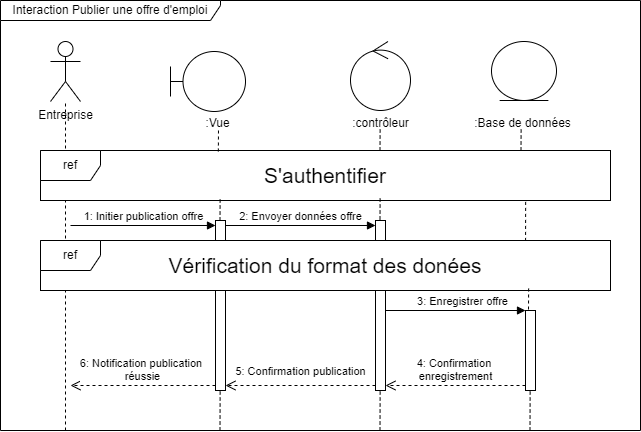
\includegraphics[width=0.8\textwidth]{images/PublierOffreEmploiSequencefinale1.drawio.png}
    \caption{Diagramme des Séquence Publier une offre d'emploi}
    \label{fig:publier_offre_emploi}
\end{figure}

\subsection{Diagrammes de séquence - Projets Freelance}
\subsubsection{Diagramme de séquence de "Publier un projet freelance"}
La figure 5.8 présente le diagramme de séquence du cas d'utilisation "Publier un projet freelance".

% Insérer ici l'image du diagramme de séquence
\begin{figure}[H]
    \centering
    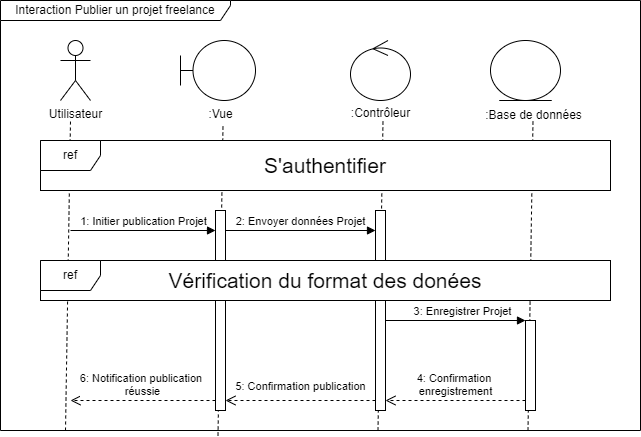
\includegraphics[width=0.8\textwidth]{images/PublierProjetFreelanceseq.png}
    \caption{Diagramme de séquence Publier Un Projet freelance}
    \label{fig:publier_projet_freelance}
\end{figure}
\subsubsection{Diagramme de séquence de "Soumettre une condidature pour un projet"}
La figure 5.9 présente le diagramme de séquence du cas d'utilisation "Soumettre une condidature pour un projet".

% Insérer ici l'image du diagramme de séquence
\begin{figure}[H]
    \centering
    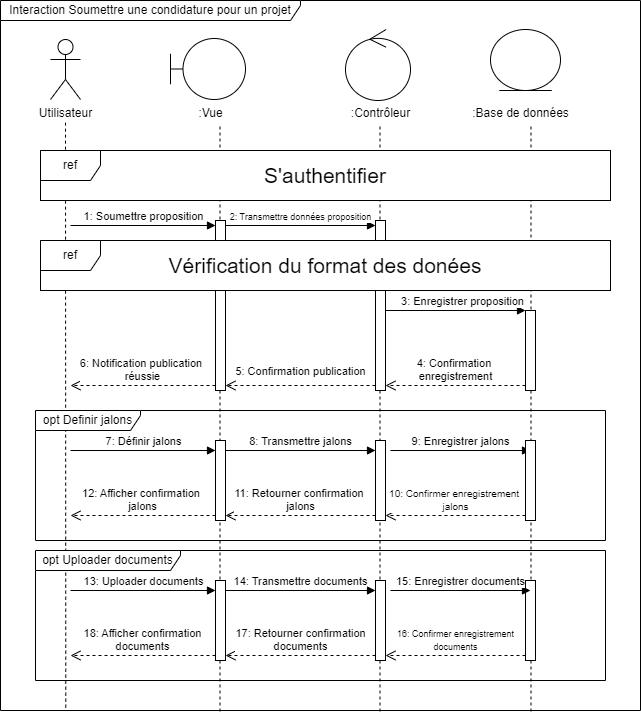
\includegraphics[width=0.8\textwidth]{images/SoumettreunePepSeqequence.drawio.png}
    \caption{Diagramme de séquence Soumettre une condidature pour un projet freelance}
    \label{fig:postuler_projet_freelance}
\end{figure}

%\subsubsection{Diagramme de séquence de "Gérer les contrats"}
%La figure 5.12 présente le diagramme de séquence du cas d'utilisation "Gérer les contrats".

% Insérer ici l'image du diagramme de séquence
%\begin{figure}[H]
%    \centering
%    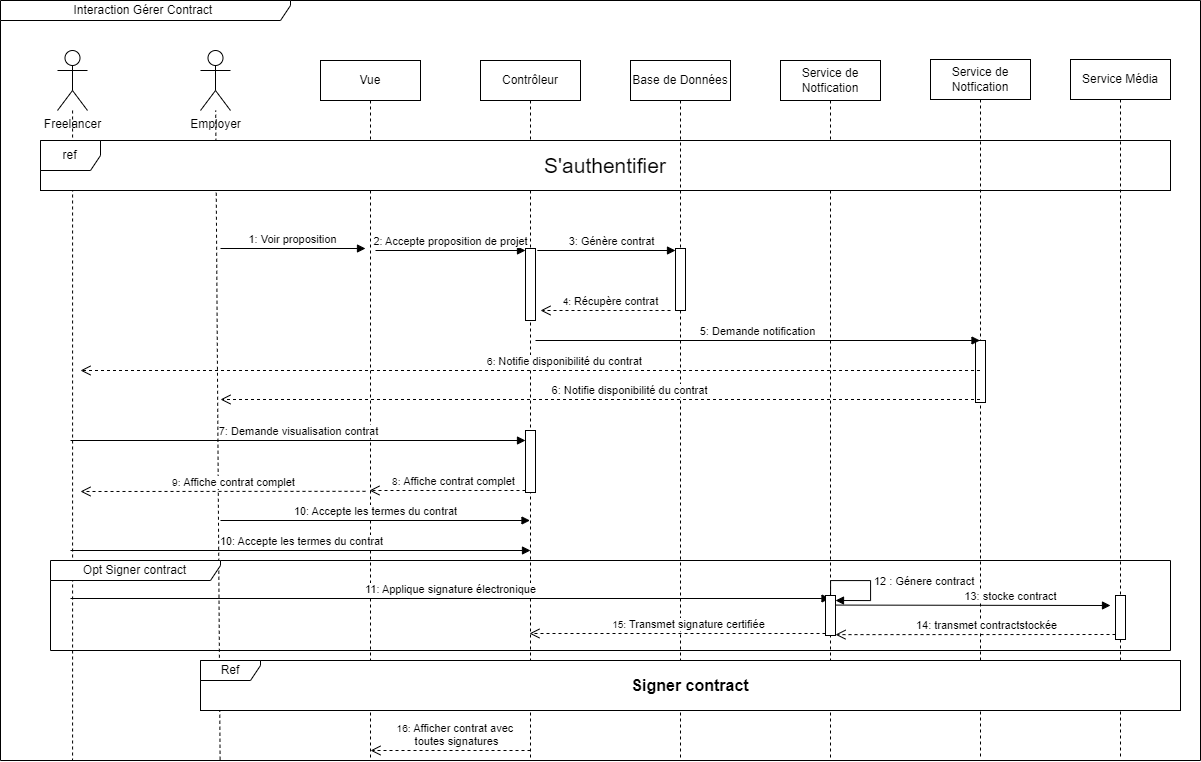
\includegraphics[width=0.8\textwidth]{images/GérerContractSéq.png}
 %   \caption{Diagramme de séquence Gérer les contrats}
 %   \label{fig:gerer_contrats_sequence}
%\end{figure}
\subsection{Diagrammes de séquence - Messagerie}
\subsubsection{Diagramme de séquence de "Envoyer un message direct"}
La figure 5.10 présente le diagramme de séquence du cas d'utilisation "Envoyer un message direct".

% Insérer ici l'image du diagramme de séquence
\begin{figure}[H]
    \centering
    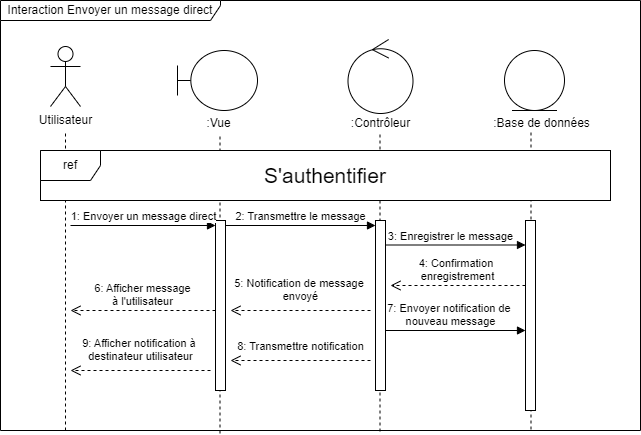
\includegraphics[width=0.8\textwidth]{images/Envoyer un message direct Sequencefinale1.drawio.png}
    \caption{Diagramme de séquence Envoyer un message direct}
    \label{fig:Envoyer_un_message_direct}
\end{figure}
\subsubsection{Diagramme de séquence de "Créer une conversation de groupe"}
La figure 5.11 présente le diagramme de séquence du cas d'utilisation "Créer une conversation de groupe".

% Insérer ici l'image du diagramme de séquence
\begin{figure}[H]
    \centering
    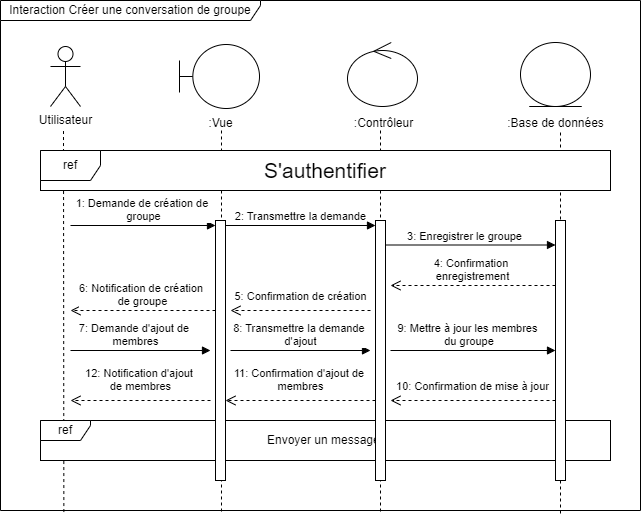
\includegraphics[width=0.8\textwidth]{images/Créer une conversation de groupe Sequence.drawio.png}
    \caption{Diagramme de séquence Créer une conversation de groupe}
    \label{fig:créer_conversation}
\end{figure}
\subsection{Diagrammes d'activité - Signer un contract}
\paragraph{Diagramme d'activité pour le signature}
Nous choisissons de réaliser un diagramme d'activité dans la figure 5.12 afin d'illustrer de manière claire et structurée les différentes étapes du processus de génération et de signature électronique du contrat.
\begin{figure}[H]
    \centering
    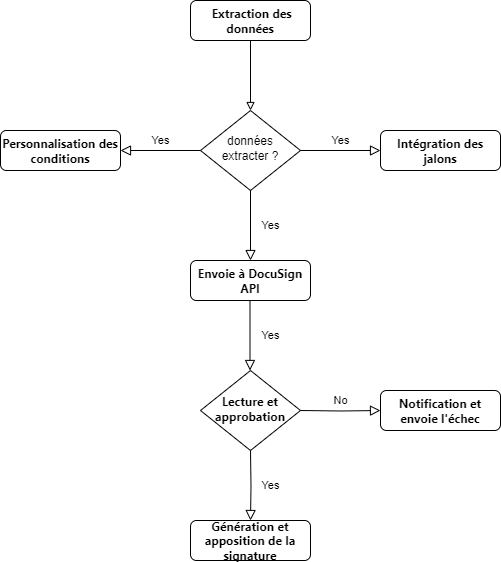
\includegraphics[width=0.8\textwidth]{images/DiagrammeFluxSignature.png}
    \caption{Diagrammes d'activité - Signer un contract}
    \label{fig:gerer_contrats_flux}
\end{figure}
\section{Réalisation du sprint 5}
\subsection{Architecture générale}
Pour la réalisation du sprint 5, nous avons conservé l'architecture microservices mise en place dans les sprints précédents, en y ajoutant les nouveaux microservices nécessaires pour gérer les offres d'emploi, les projets freelance et la messagerie. Chaque microservice est responsable d'une fonctionnalité spécifique et communique avec les autres via des API REST et des événements asynchrones.

\subsection{Réalisation du module Offres d'emploi}
Le module d'offres d'emploi a été implémenté avec un microservice dédié qui gère la création, la modification, la recherche et la candidature aux offres d'emploi. Les principales fonctionnalités développées incluent :
\begin{itemize}
    \item La publication d'offres d'emploi avec géolocalisation
    \item La recherche avancée avec filtres et rayons de distance
    \item Le système de candidature avec upload de documents
    \item La gestion des statuts des candidatures
    \item Le système de notification pour les mises à jour de statut
\end{itemize}

\subsection{Réalisation du module Projets Freelance}
Le module de projets freelance a été développé comme un service distinct, assurant l'ensemble du cycle de vie des projets, depuis leur publication jusqu'à la contractualisation. Les principales fonctionnalités mises en œuvre sont :
\begin{itemize}
    \item La création de projets avec spécifications détaillées
    \item Le système de proposition avec jalons et documents
    \item La gestion des propositions reçues
    \item La génération et signature électronique de contrats
    \item Le système de notification pour le suivi des projets
\end{itemize}

\subsubsection{Focus sur le Système de Contrats}

Le système de contrats constitue un élément central du module \textit{Projets Freelance}, assurant la sécurisation des accords entre employeurs et freelances. Sa conception robuste garantit la validité juridique des engagements tout en offrant une expérience utilisateur fluide et conforme aux standards internationaux.

\paragraph{La signature électronique :}

La signature électronique est un procédé numérique permettant d'authentifier un document de manière sécurisée et juridiquement reconnue. Elle garantit que le document signé provient bien du signataire et qu'il n'a pas été altéré depuis la signature. La signature électronique repose sur des technologies cryptographiques, comme la clé publique/clé privée, assurant ainsi la confidentialité, l'intégrité et la non-répudiation du document. Grâce à des fournisseurs de services spécialisés tels que DocuSign, la signature électronique répond aux exigences légales internationales, notamment le règlement européen eIDAS et la loi américaine ESIGN Act, conférant aux documents signés une valeur légale équivalente à une signature manuscrite traditionnelle.

\paragraph{Architecture du système de contrats}
L'architecture repose sur une intégration modulaire combinant des mécanismes de génération, de signature et de vérification des contrats. Elle s'articule autour de quatre composants clés :

\begin{itemize}
    \item \textbf{Générateur de contrats} : Moteur de création dynamique de documents juridiques basé sur des modèles prédéfinis, paramétrables selon les informations du projet (durée, montant, responsabilités, etc.).

    \item \textbf{Intégration \textbf{DocuSign} (Provider)} : Un fournisseur tiers, \textbf{DocuSign}, est intégré au système pour la gestion de la signature électronique. Il assure la conformité légale (\textbf{eIDAS, ESIGN Act}) et permet une expérience utilisateur sécurisée via une interface de confirmation et d'authentification.

    \item \textbf{Système de confirmation et de hashage} : Après validation de la signature par DocuSign, un hachage cryptographique (\textbf{SHA-1}) est généré à partir du contenu du contrat signé. Ce hash est stocké de manière immuable afin de permettre une vérification ultérieure de l'intégrité du document.

    \item \textbf{Gestionnaire de cycle de vie des contrats} : Ce composant assure le suivi des statuts (en attente, signé, expiré), l'archivage sécurisé, ainsi que la consultation des historiques. Il garantit la traçabilité et la conservation des contrats dans le temps.
\end{itemize}

\paragraph{Sécurité et conformité}
Ce système garantit :
\begin{itemize}
    \item la \textbf{valeur légale} des signatures via l'utilisation de DocuSign comme autorité de confiance,
    \item la \textbf{non-répudiation} grâce au stockage du hash unique de chaque contrat,
    \item et la \textbf{traçabilité} complète à travers des journaux d'activité et des horodatages précis.
\end{itemize}


\begin{figure}[H]
    \centering
    % Si vous créez cette image, vous pouvez décommenter la ligne suivante
    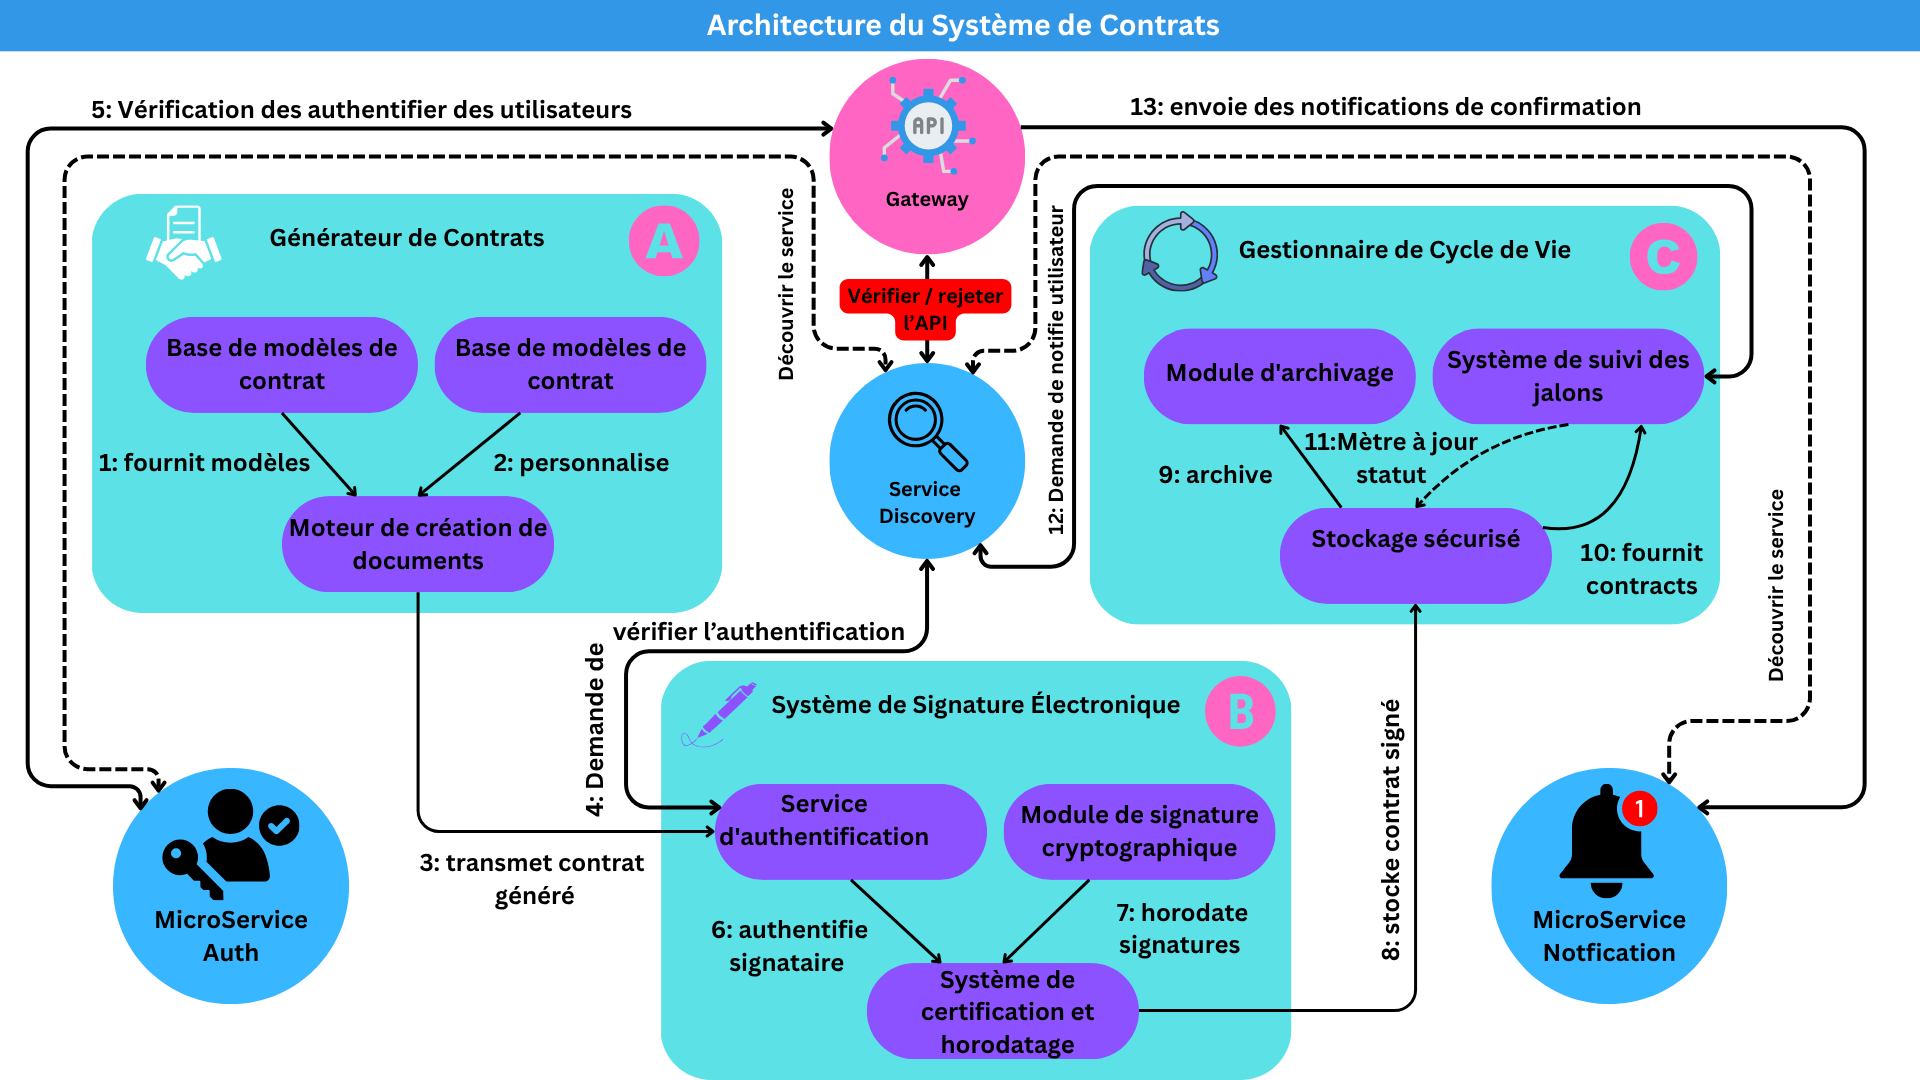
\includegraphics[width=0.9\textwidth]{images/ArchContractv2.png}
    \caption{Architecture du système de contrats}
    \label{fig:architecture_contrats}
\end{figure}

\paragraph{Génération automatique de contrats}
Le processus de génération de contrats s'effectue en plusieurs étapes :

\begin{enumerate}
    \item Extraction des données du projet et de la proposition acceptée (budget, délais, livrables)
    \item Intégration des jalons définis par le freelance dans l'échéancier contractuel
    
    \item Personnalisation des conditions spécifiques (modalités de paiement, propriété intellectuelle)
    \item Compilation en document PDF sécurisé avec métadonnées d'identification uniques
\end{enumerate}

Les contrats générés incluent automatiquement :
\begin{itemize}
    \item Un descriptif détaillé des prestations
    \item Le calendrier précis avec jalons et livrables
    \item Les modalités de paiement et d'exécution
    \item Les clauses de confidentialité et de propriété intellectuelle
    \item Les conditions de résiliation et de règlement des litiges
\end{itemize}

\paragraph{Signature électronique sécurisée}
Le système de signature électronique implémenté respecte les standards internationaux et offre une valeur juridique équivalente à une signature manuscrite. Ses caractéristiques principales sont :

\begin{itemize}
   
    \item \textbf{Piste d'audit complète} : Enregistrement horodaté de toutes les actions (création, envoi, visualisation, signature)
    
    \item \textbf{Certificats numériques} : Utilisation de certificats cryptographiques pour garantir l'authenticité des signataires
    
    \item \textbf{Validation visuelle} : Apposition d'un sceau visible sur le document avec informations sur le signataire
\end{itemize}

Le processus de signature se déroule comme suit :

\begin{enumerate}
    \item Notification aux parties (employeur et freelance) de la disponibilité du contrat
    \item Authentification sécurisée de chaque partie
    \item Présentation du contrat avec possibilité de lecture complète
 
    \item Émission d'un certificat de signature et horodatage cryptographique
    \item Distribution du document final signé aux parties concernées
\end{enumerate}

\begin{figure}[H]
    \centering
    % Si vous créez cette image, vous pouvez décommenter la ligne suivante
     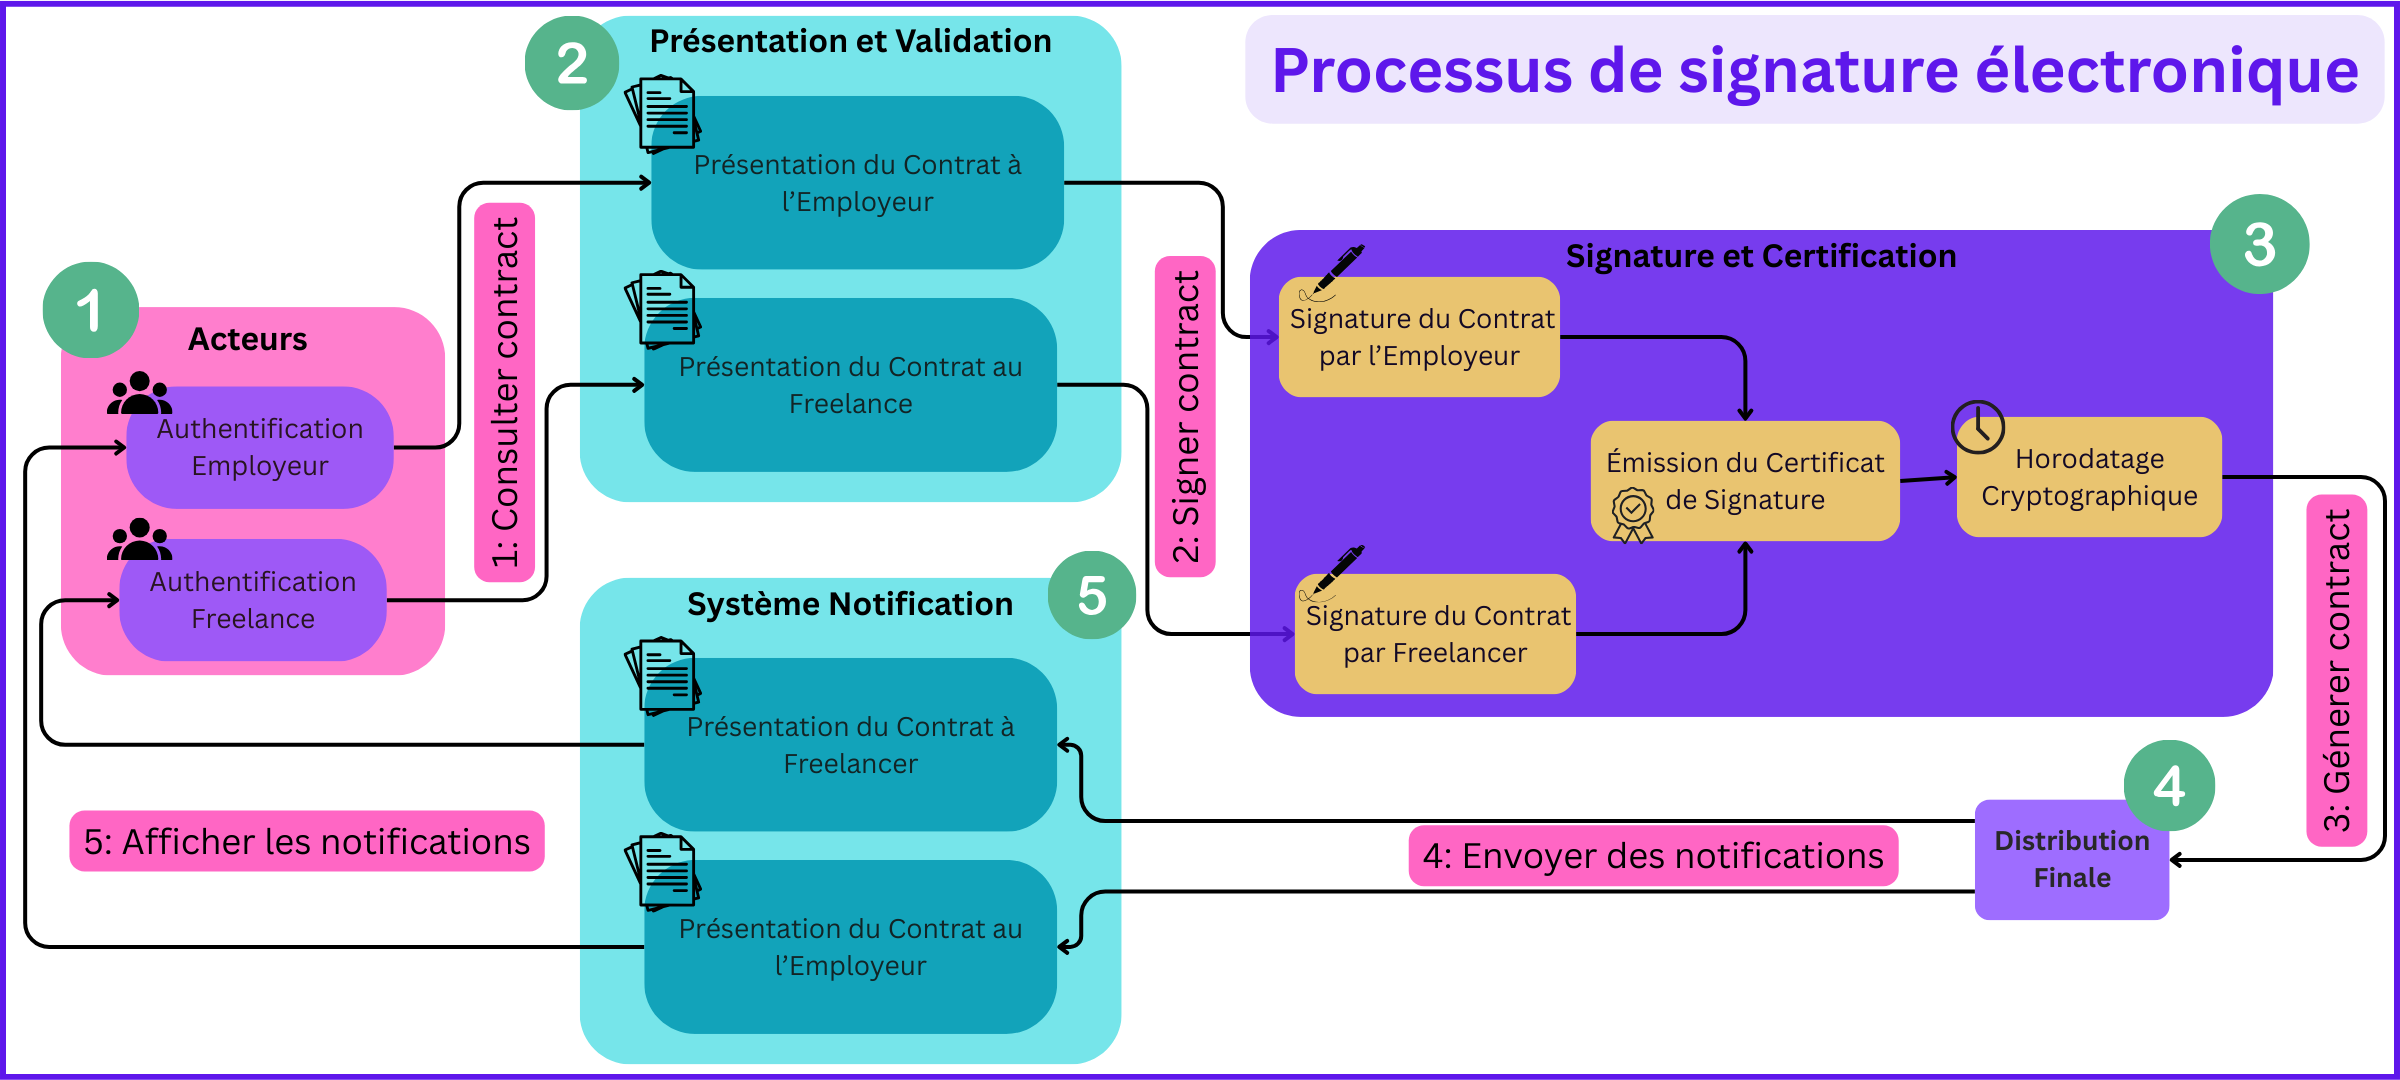
\includegraphics[width=\textwidth]{images/processus_signature.png}
    \caption{Processus de signature électronique}
    \label{fig:processus_signature}
\end{figure}

\paragraph{Gestion du cycle de vie des contrats}
Après la signature, le système assure un suivi complet du cycle de vie contractuel :

\begin{itemize}
    \item \textbf{Stockage sécurisé} : Conservation des contrats dans un système chiffré avec redondance
    
    \item \textbf{Suivi des jalons} : Monitoring automatique des échéances définies et génération de notifications
    
    \item \textbf{Gestion des avenants} : Possibilité de modifier le contrat par accord mutuel avec traçabilité complète
    
\end{itemize}

\paragraph{Sécurité et confidentialité}
Le système de contrats intègre des mesures de sécurité avancées :

\begin{itemize}
    \item Chiffrement des liens en URL signé pour tous les documents
    \item Contrôle d'accès granulaire basé sur les rôles
    \item Protection contre les modifications non autorisées via hachage 
  
\end{itemize}

\paragraph{Intégration avec les autres modules}
Le système de contrats s'intègre de manière transparente avec :

\begin{itemize}
    \item Le module de gestion de projets pour synchroniser l'avancement des livrables
    \item Le système de notification pour les rappels d'échéances et d'obligations
\end{itemize}

Cette approche intégrée offre une expérience fluide aux utilisateurs tout en garantissant les éléments fondamentaux pour établir la confiance dans un environnement de travail freelance.

\subsection{Réalisation du module Messagerie}
Le module de messagerie a été implémenté comme un service en temps réel utilisant des technologies de WebSocket pour assurer une communication instantanée. Les principales fonctionnalités développées comprennent :
\begin{itemize}
    \item L'échange de messages directs entre utilisateurs
    \item La création et gestion de conversations de groupe et direct
    \item Le partage de médias et documents
    \item Le système de notification pour les nouveaux messages
    \item La gestion des statuts de lecture des messages
\end{itemize}




\section{Technologies et Outils Utilisés}
Dans le cadre du sprint 5 dédié au développement des modules d'offres d'emploi, projets freelance et messagerie, nous avons employé plusieurs technologies spécialisées pour réaliser nos objectifs. Voici les principaux composants techniques qui ont permis le développement de ces fonctionnalités :


\begin{tabular}{| m{2.5cm} | m{13cm} |}
\hline


\includegraphics[width=2cm]{images/pino.png} & 
\textbf{Pino : \cite{pino}}  
Logger performant pour Node.js utilisé pour la journalisation des événements serveur, facilitant le débogage et le suivi des activités système.
\\
\hline


\includegraphics[width=2cm]{images/websocket.png} & 
\textbf{WebSocket : \cite{websocket}}  
Technologie de communication bidirectionnelle en temps réel implémentée pour notre système de messagerie, permettant l'envoi instantané des messages et des notifications aux utilisateurs connectés.
\\
\hline


\includegraphics[width=2cm]{images/pdfjs.png} & 
\textbf{PDF.js : \cite{pdfjs}}  
Bibliothèque JavaScript utilisée pour la génération et la manipulation des contrats au format PDF, permettant la création dynamique de documents juridiques personnalisés.
\\
\hline


\includegraphics[width=2cm]{images/leaflet.png} & 
\textbf{Leaflet : \cite{leaflet}}  
API de cartographie utilisée pour implémenter les fonctionnalités de géolocalisation des offres d'emploi, permettant la recherche par rayon de distance et la visualisation des opportunités sur une carte interactive.
\\
\hline
\end{tabular}
\section{Présentation des interface de l'application}
\newpage
\begin{figure}[H]
    \centering
    % Mobile interface below (centered smaller image)
    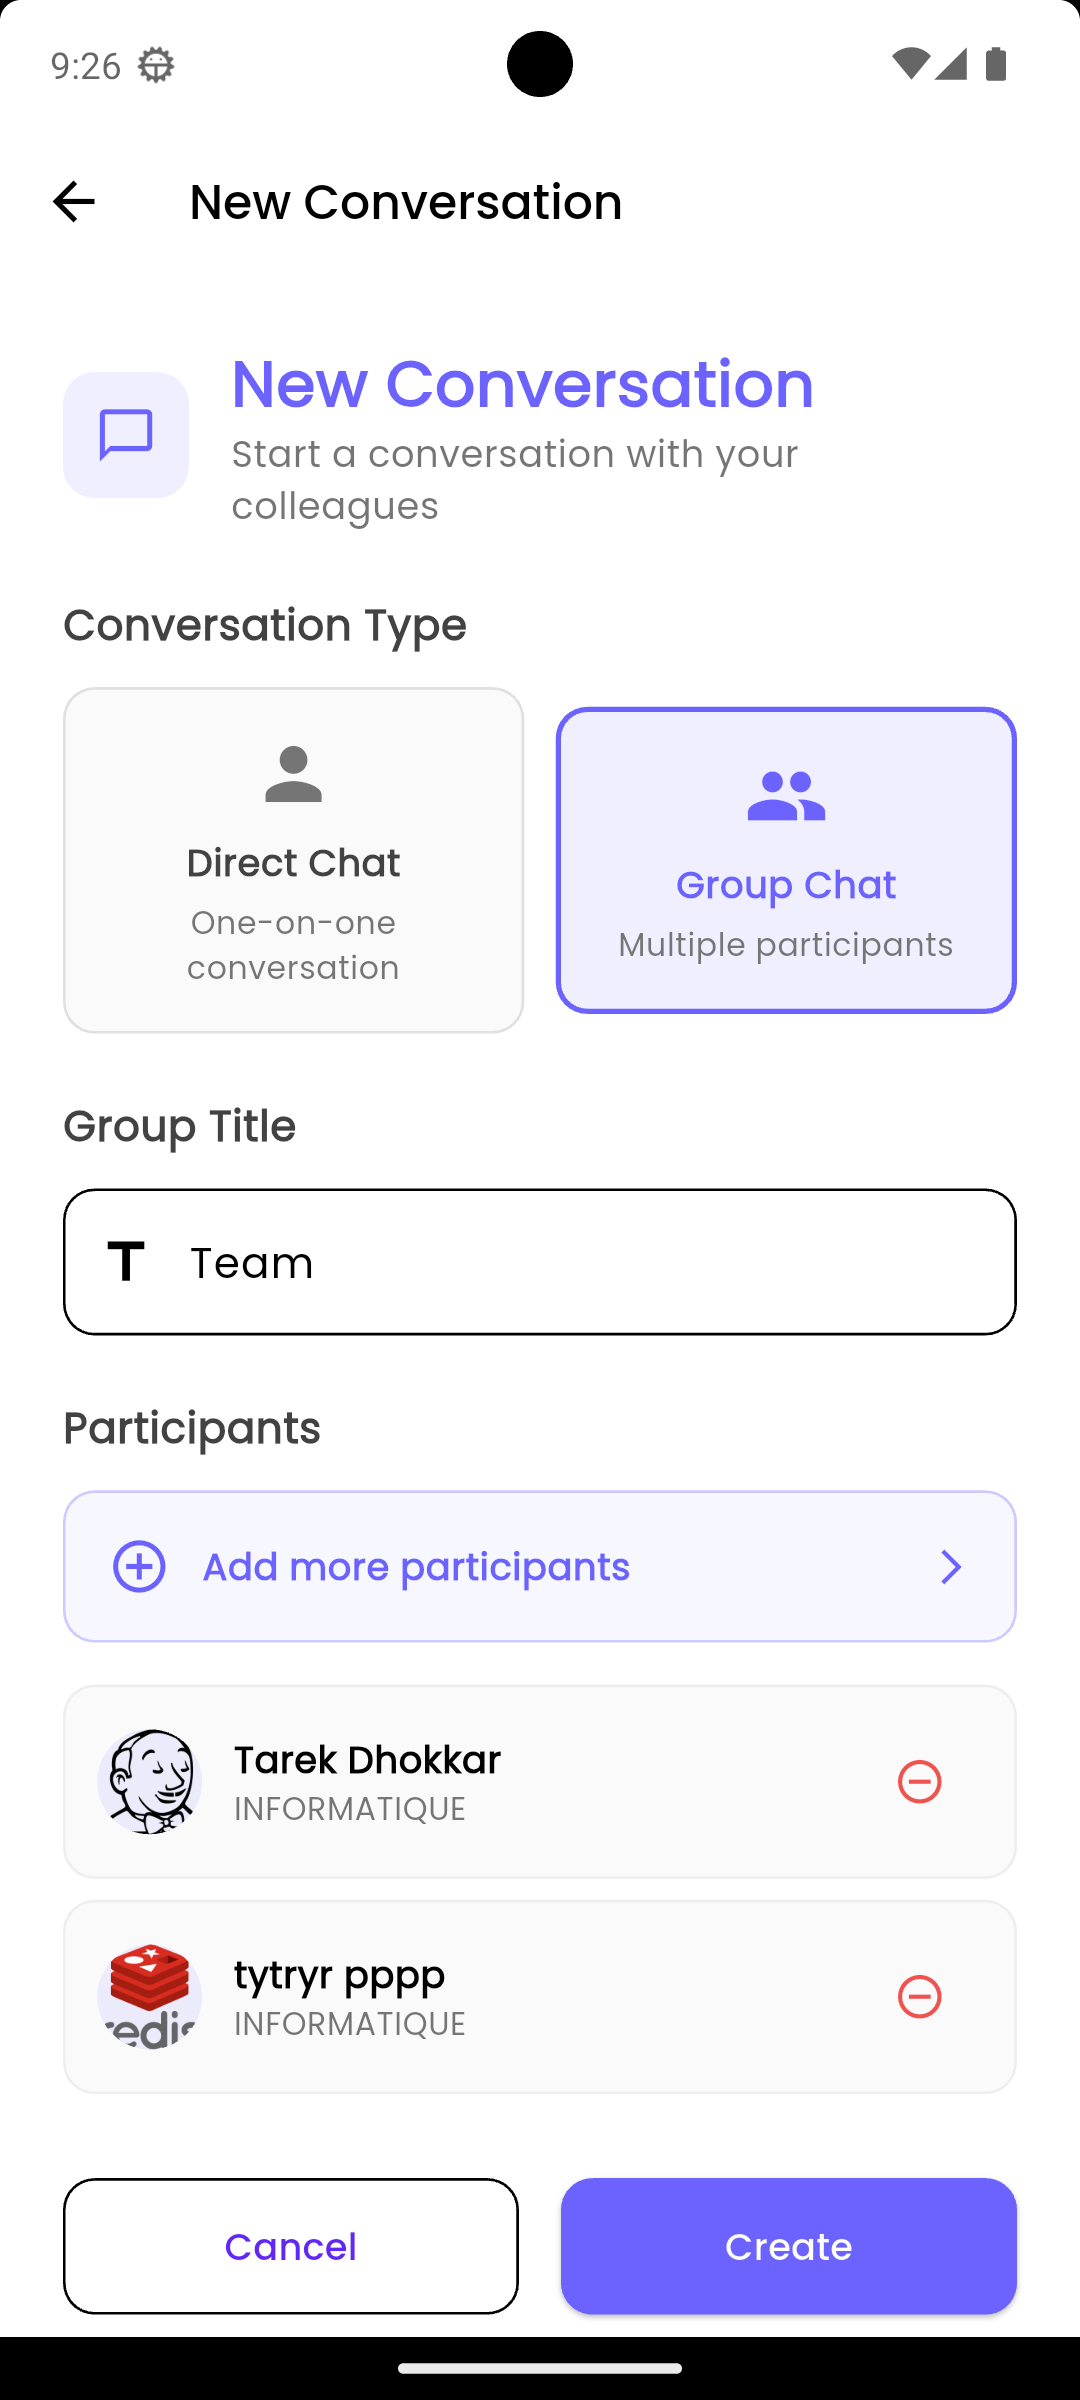
\includegraphics[width=0.35\textwidth]{images/créerConv.png}
    \caption{Interface Mobile —“ Création de Conversation —“ étape 1}

   
    \label{fig:web-mobile-messaging}

    \vspace{1em} % Optional vertical spacing


     % Web interface on top (full width)
    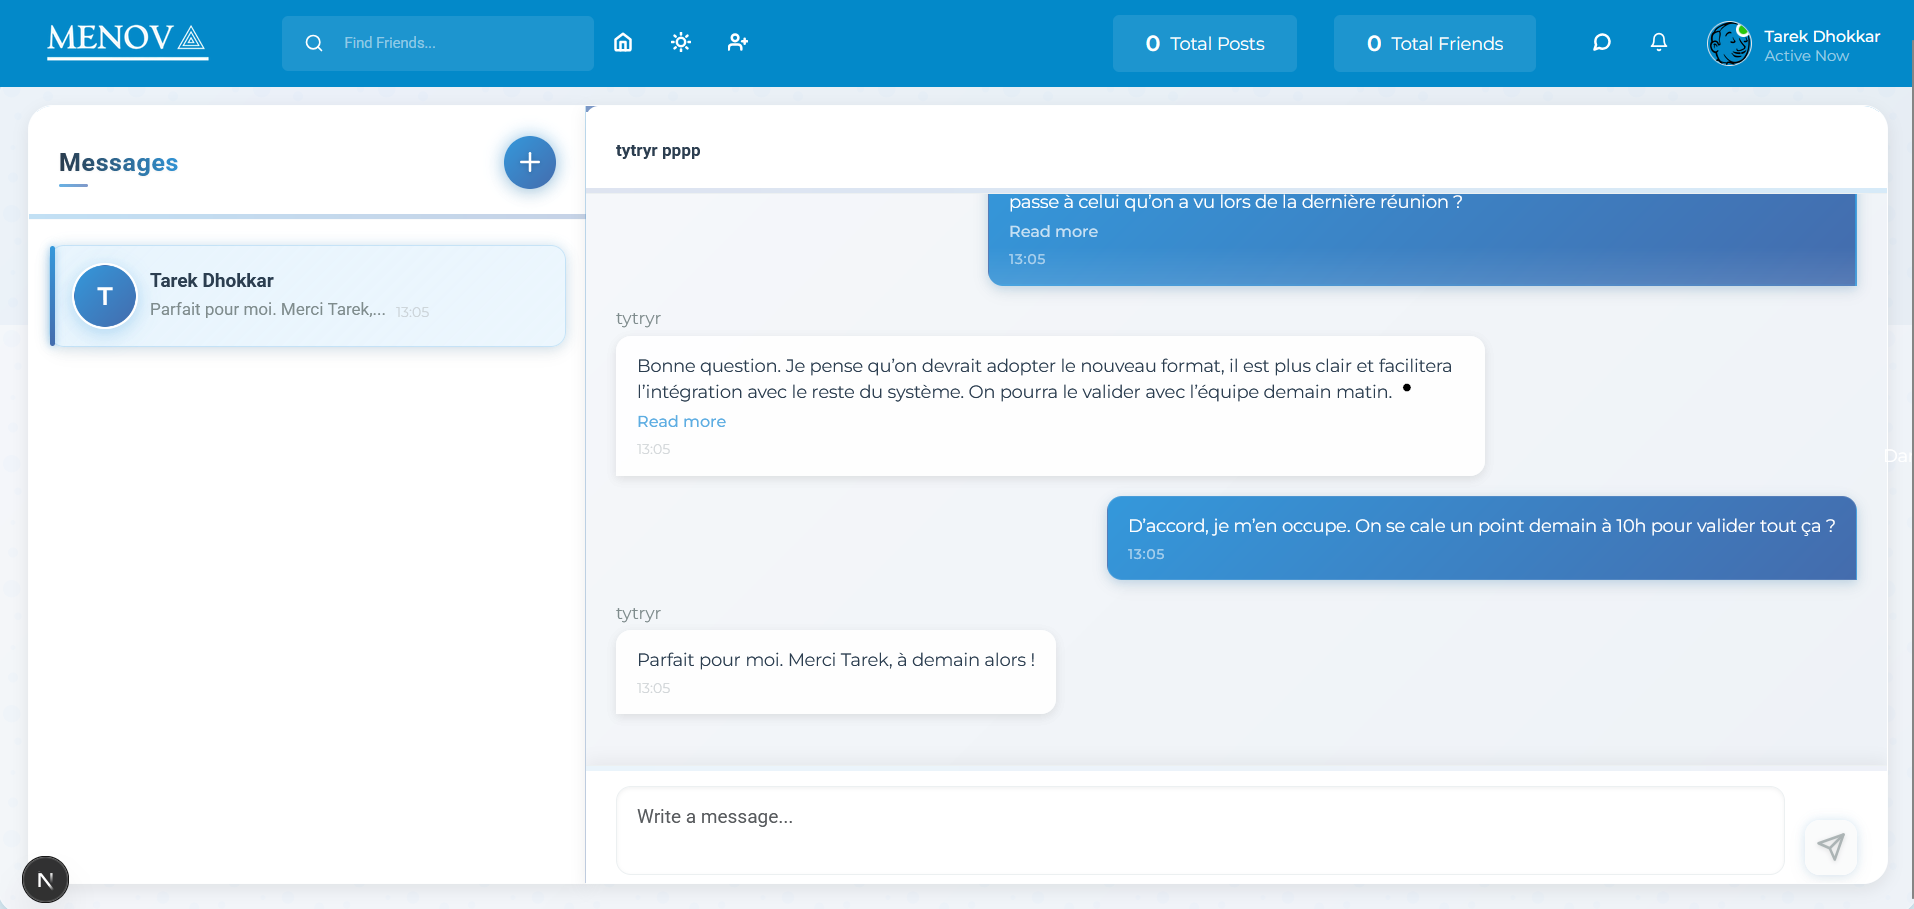
\includegraphics[width=0.9\textwidth]{Tarekconv.png}
    \caption{Interface Web —“ Messagerie —“ étape 2}
\end{figure}


\begin{figure}[H]
    \centering
    \begin{minipage}[b]{0.48\textwidth}
        \centering
        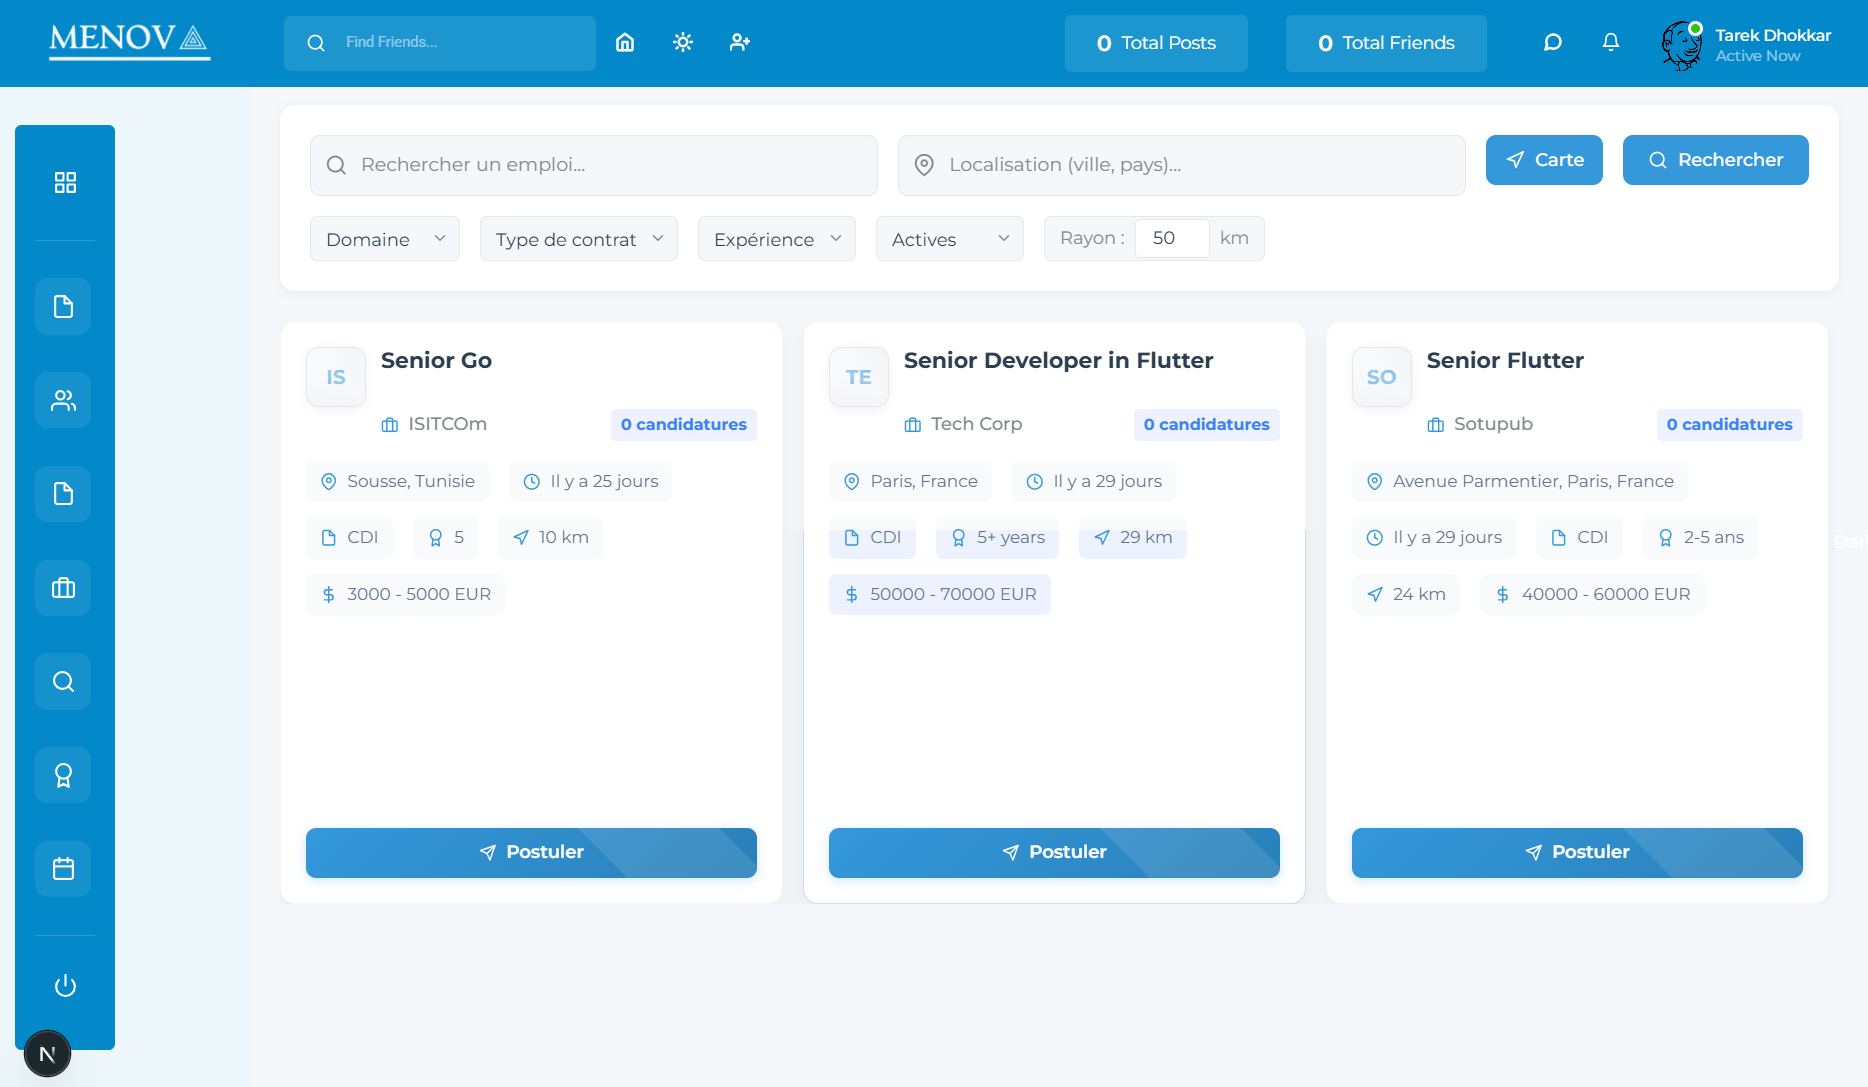
\includegraphics[width=\linewidth]{images/VoirOffres.png}
        \caption{Interface Web - Voir Offres d'emploi - étape 1}
        \label{fig:web-voir-offres}
    \end{minipage}
    \hfill
    \begin{minipage}[b]{0.48\textwidth}
        \centering
        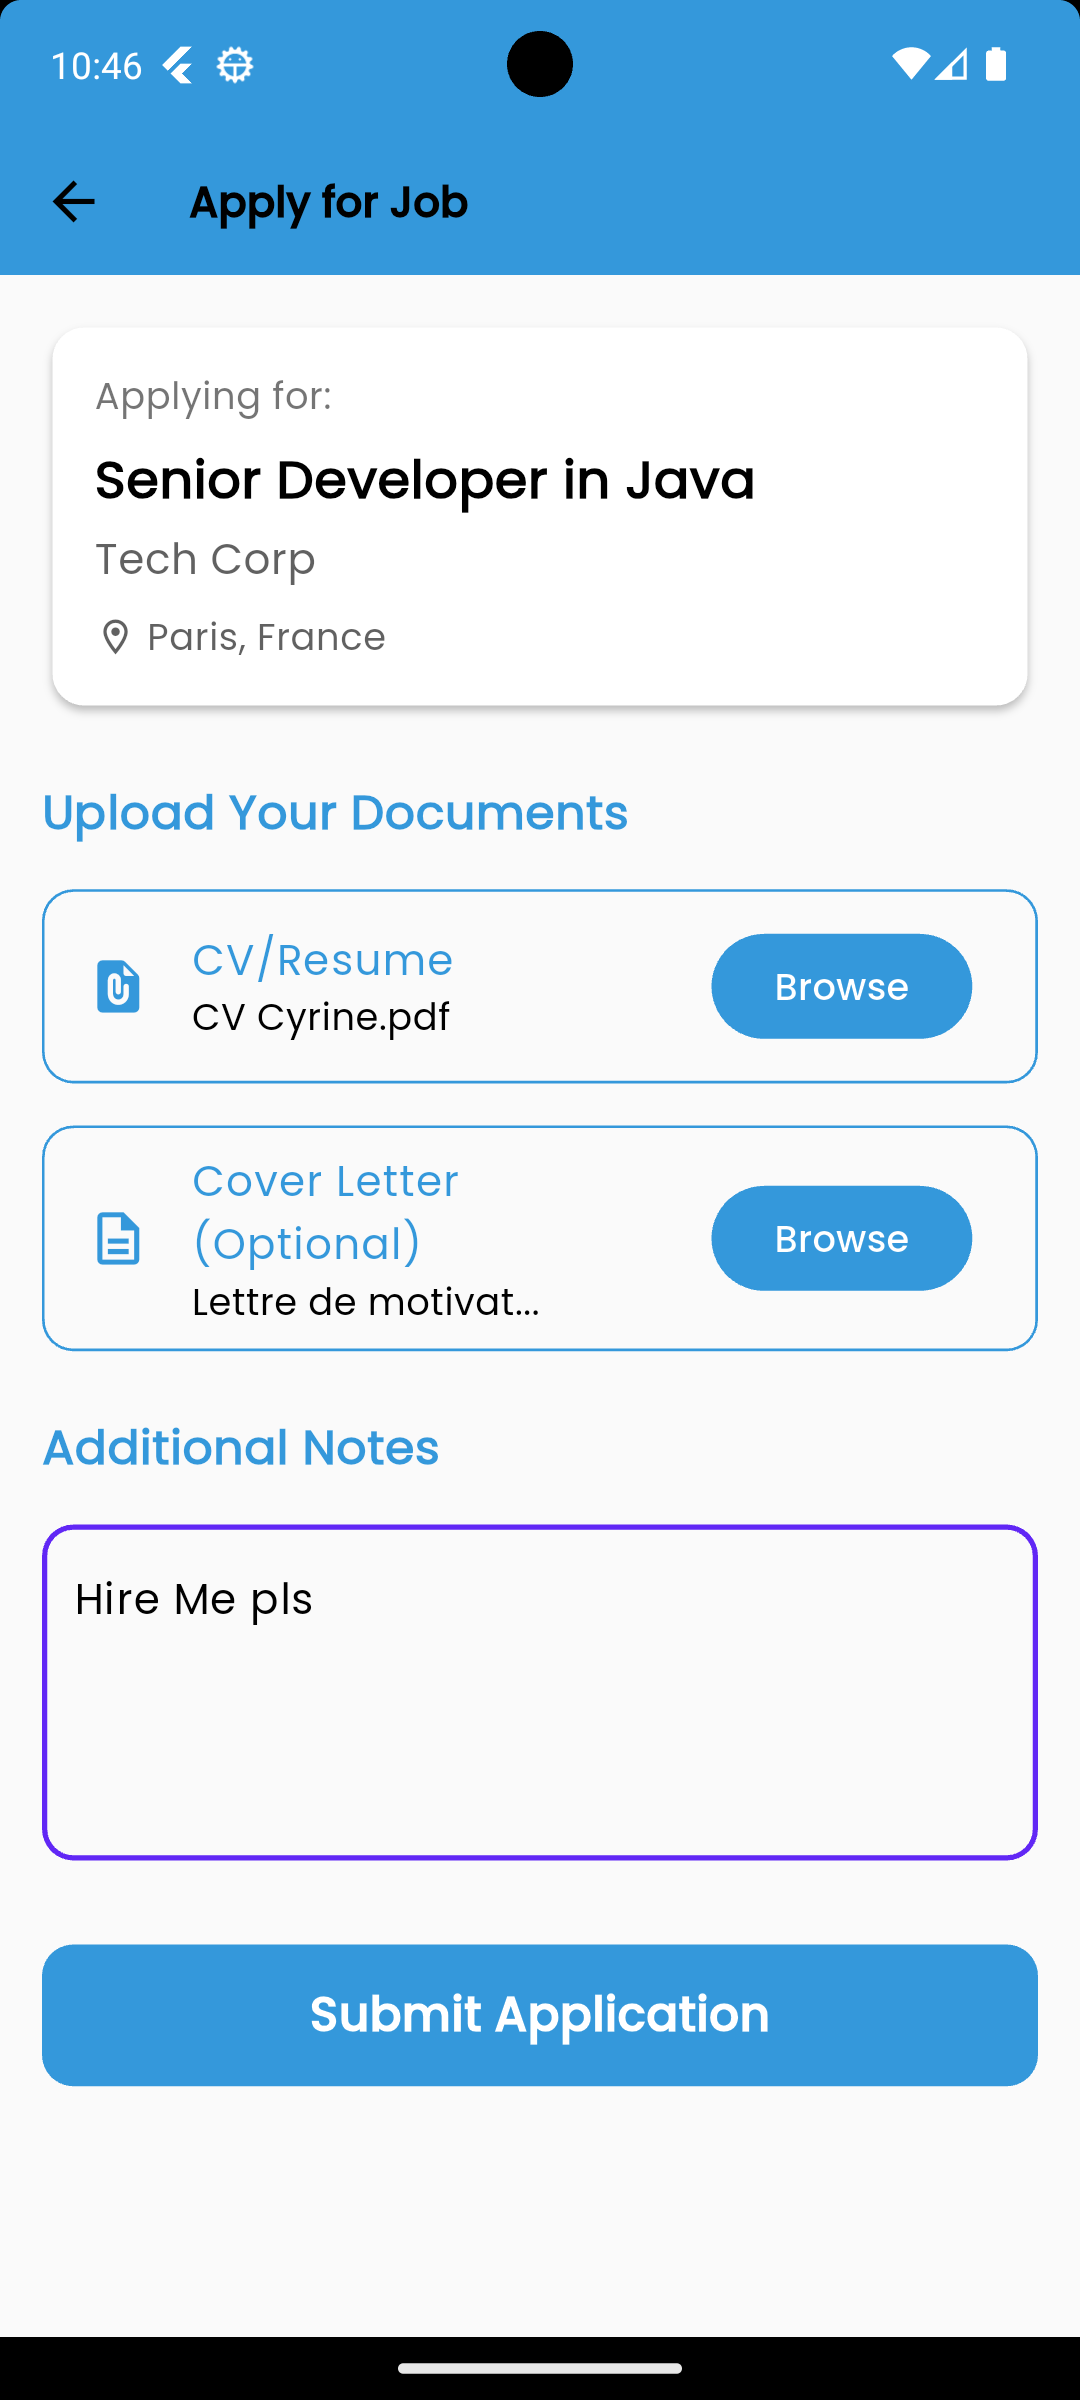
\includegraphics[height=250px]{images/mobilepostuleroffre.png}
        \caption{Interface Mobile —“ Postuler à une offre —“ étape 2}
        \label{fig:mobile-postuler}
    \end{minipage}
\end{figure}

\begin{figure}[H]
    \centering
    \begin{minipage}[b]{0.48\textwidth}
        \centering
        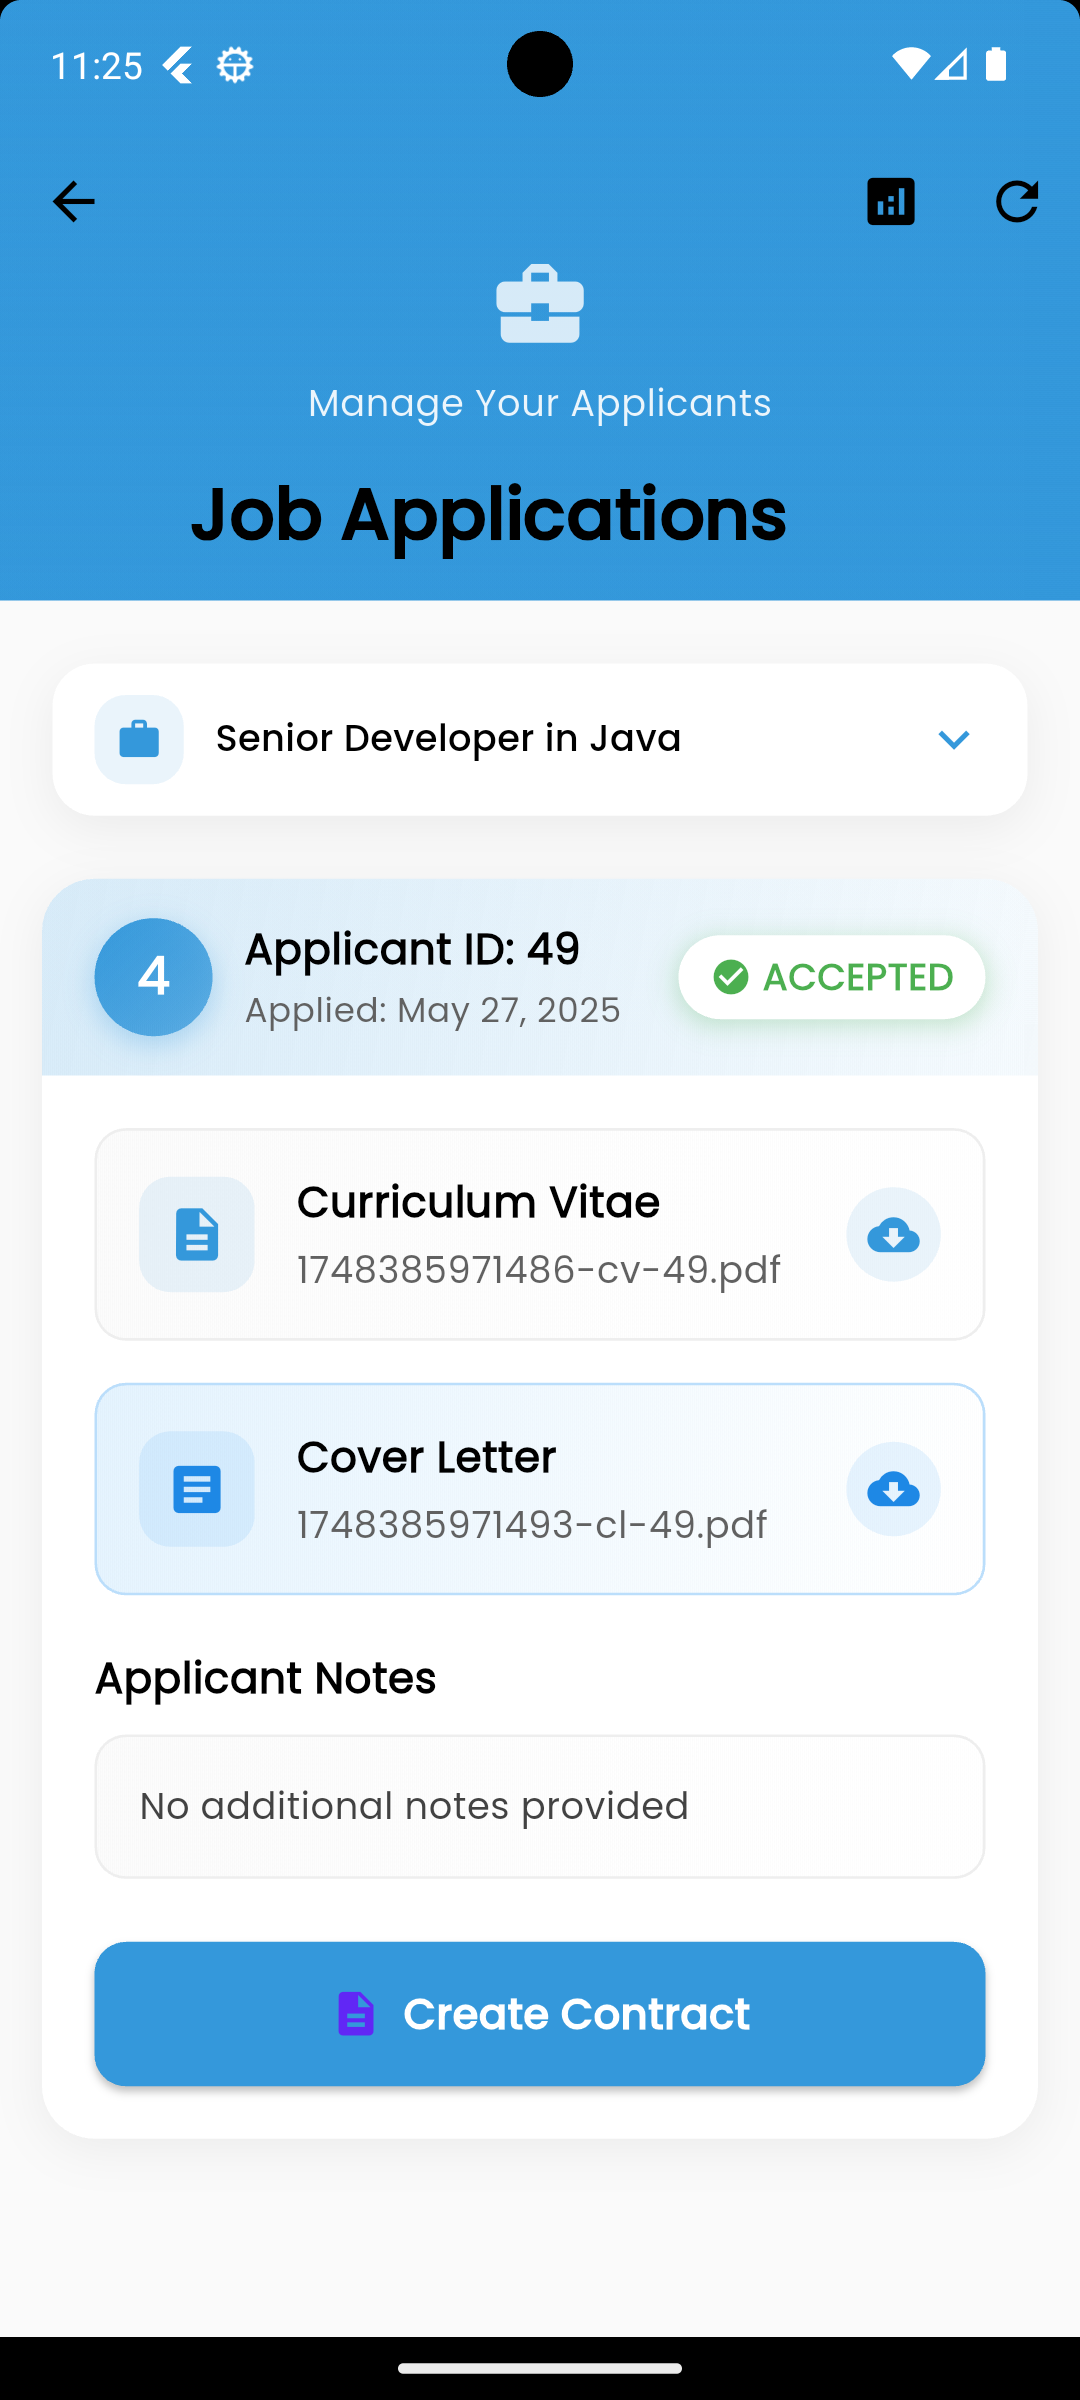
\includegraphics[height=250px]{mobilecreatecontract.png}
        \caption{Interface Mobile —“ Accepter une offre —“ étape 3}
        \label{fig:mobile-accepter}
    \end{minipage}
    \hfill
    \begin{minipage}[b]{0.48\textwidth}
        \centering
        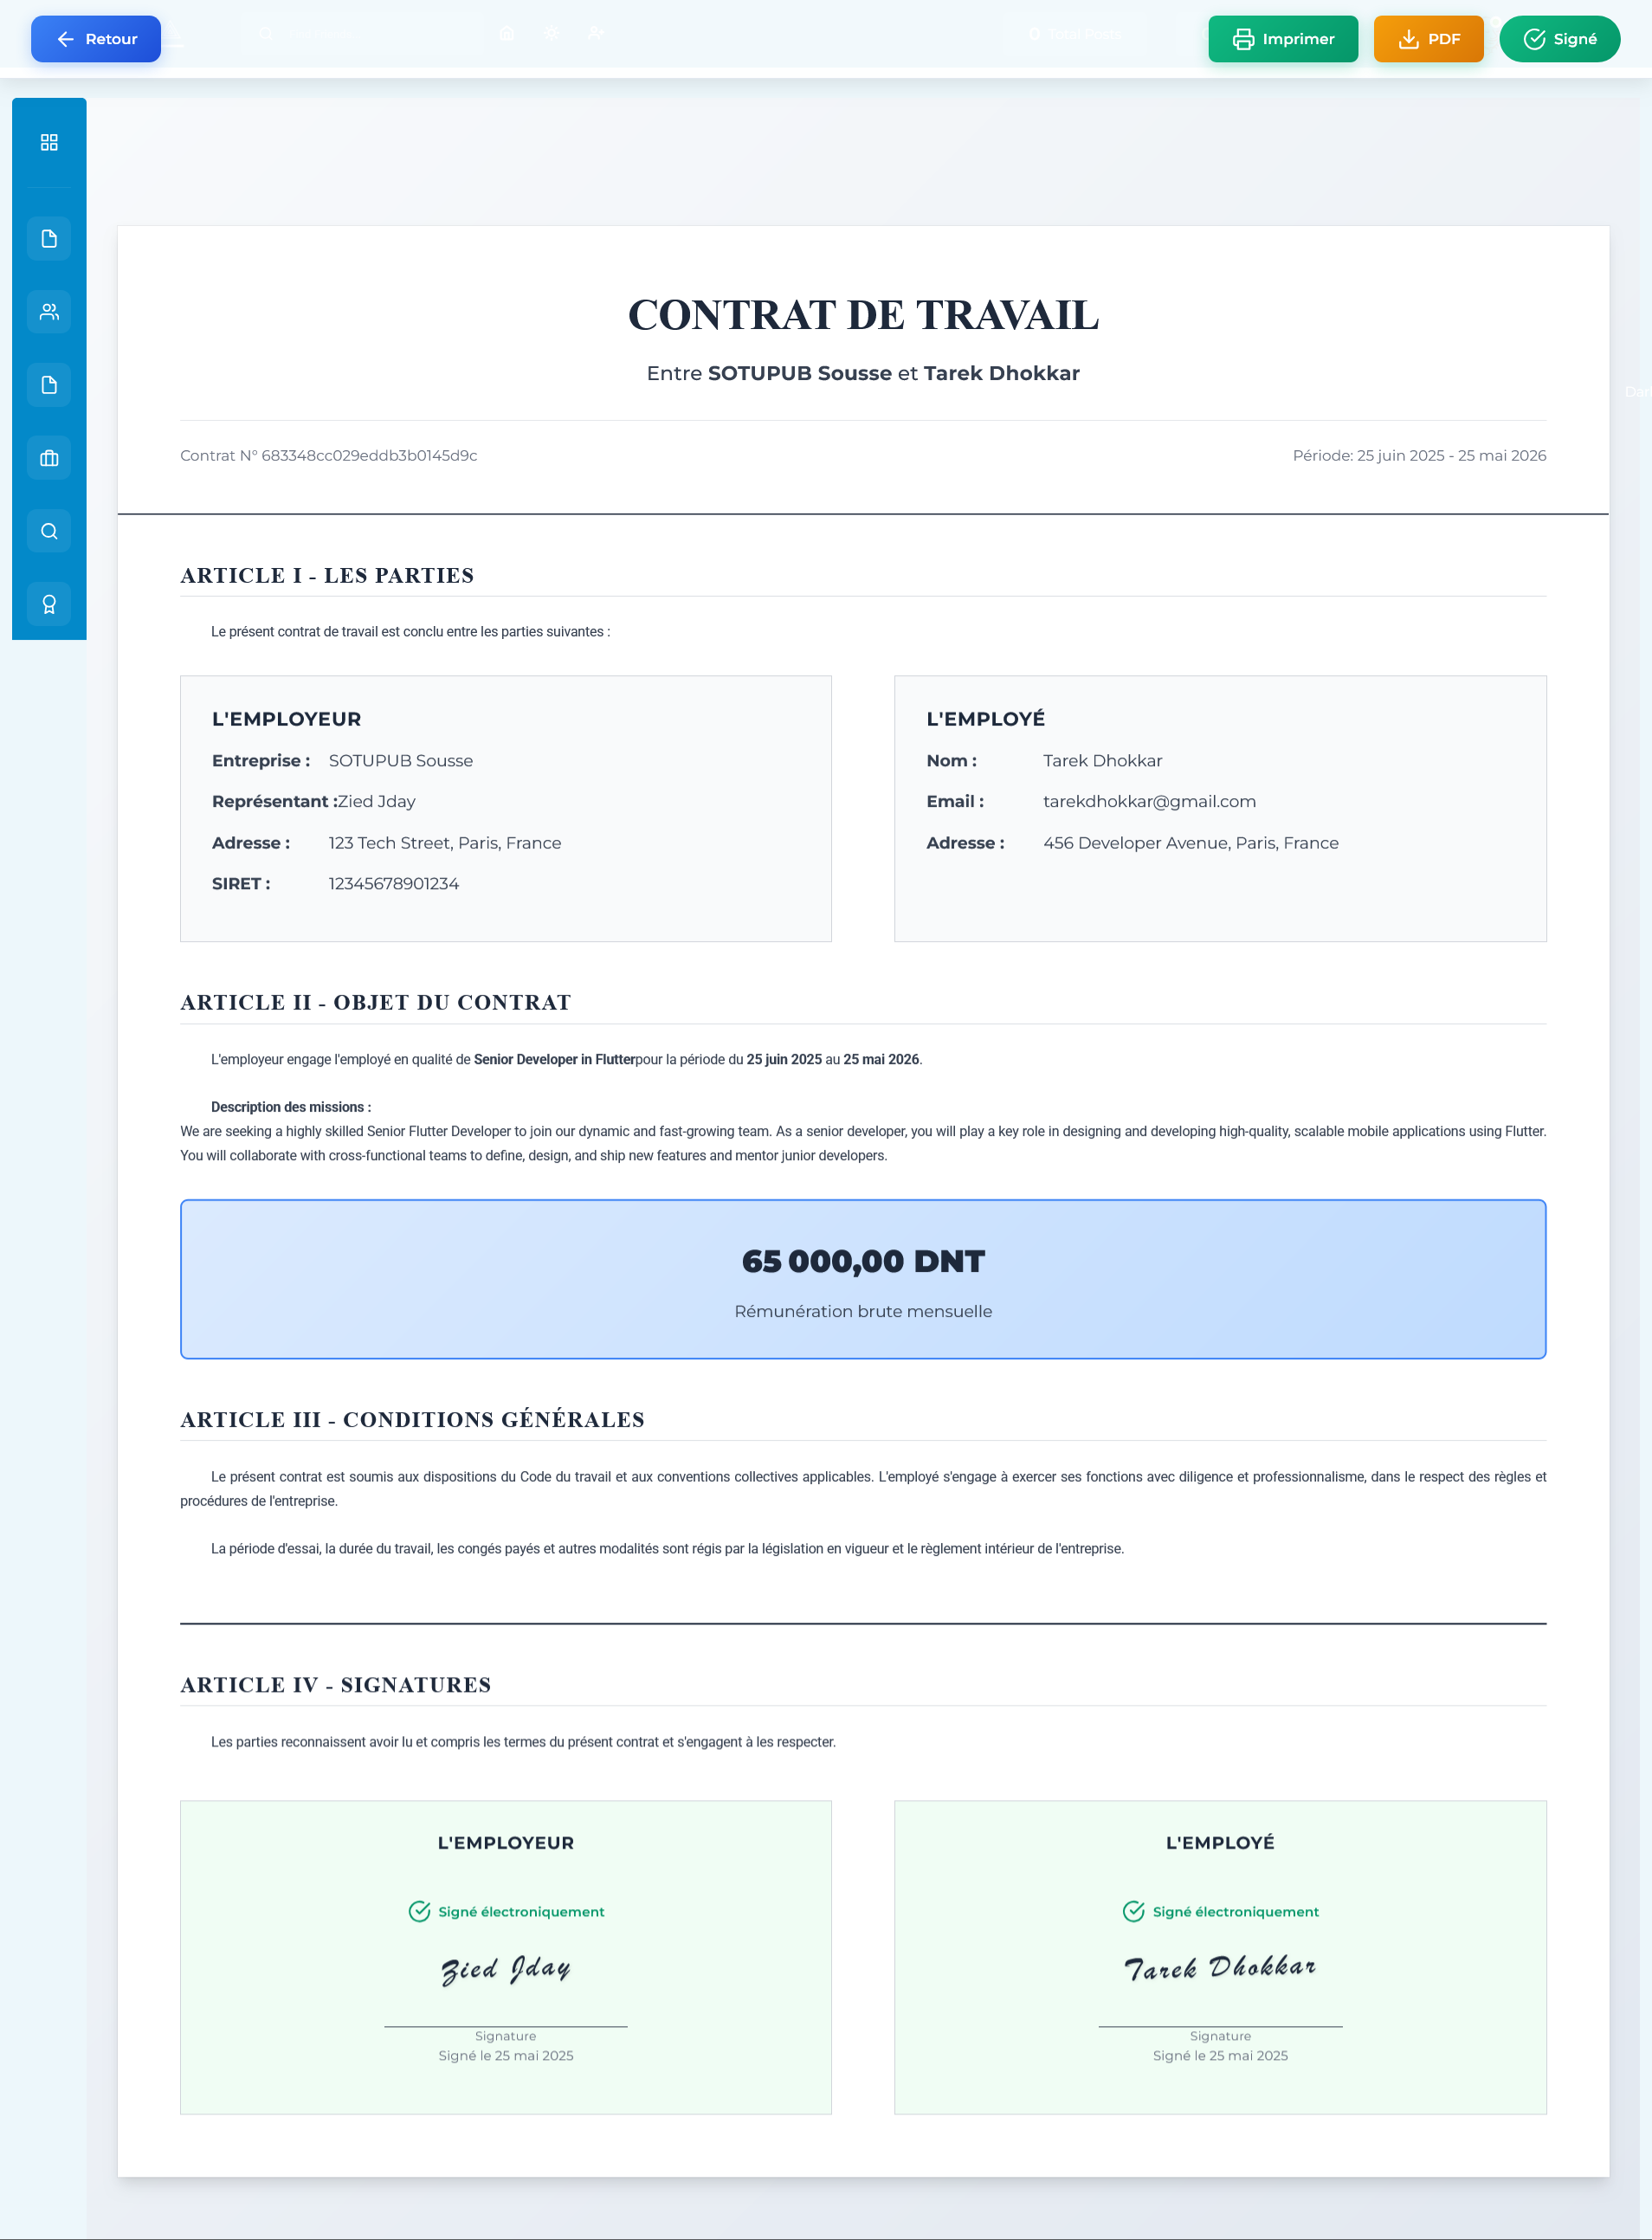
\includegraphics[width=\linewidth]{images/ContratSigned.png}
        \caption{Interface Web —“ Contrat signé —“ étape 4}
        \label{fig:web-contrat}
    \end{minipage}
\end{figure}
\begin{figure}[H]
    \centering
    % Web interface on top (full width)
    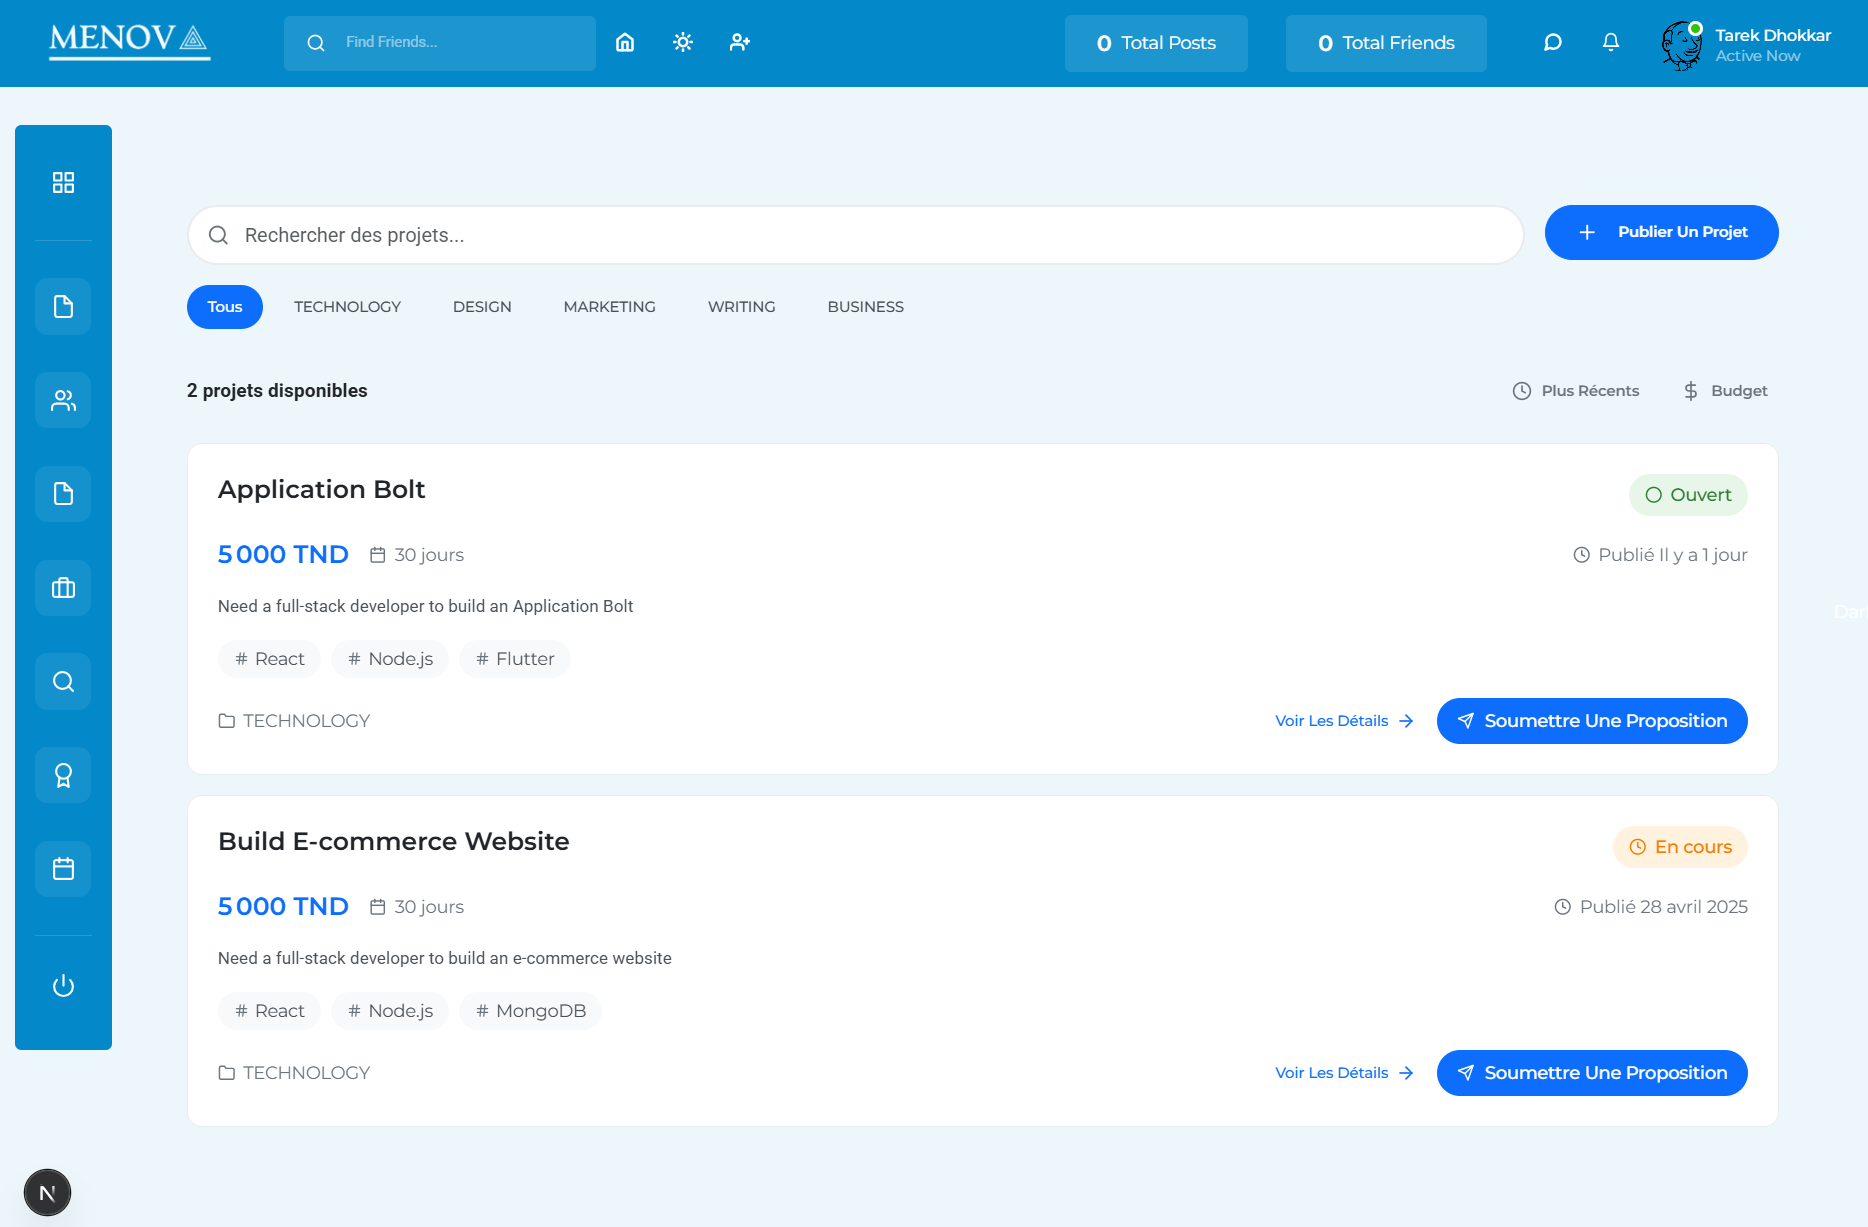
\includegraphics[width=0.8\textwidth]{images/voirprojects.png}
    \caption{Interface Web —“ Voir projects - étape 1}

    \vspace{1em} % Optional vertical spacing

    % Mobile interface below (centered smaller image)
    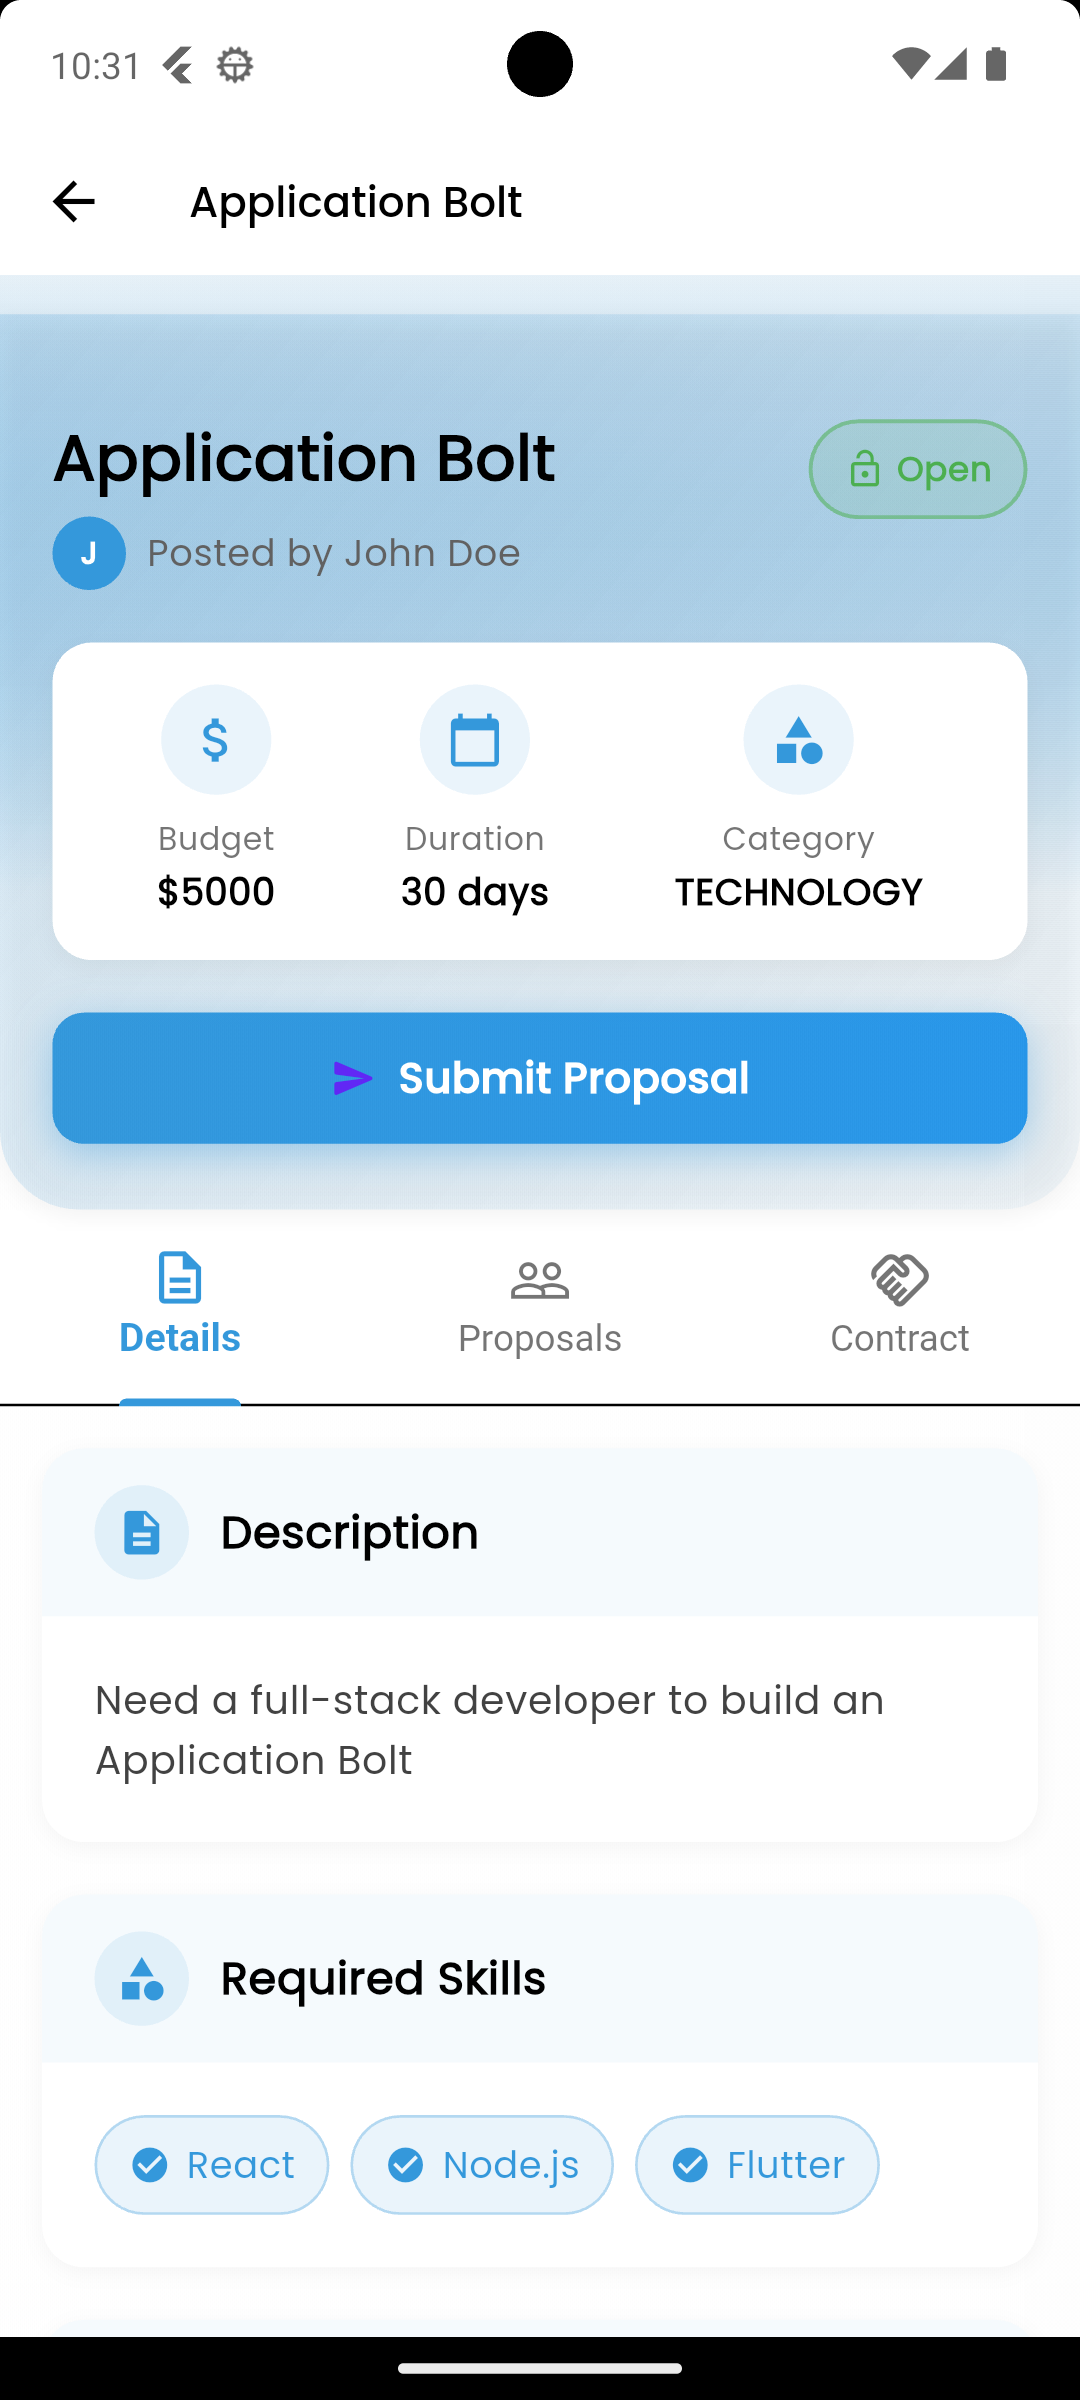
\includegraphics[width=0.35\textwidth]{images/SubmitProposalProject.png}

    \caption{Interface Mobile —“ Envoie une condidature —“ étape 2}
    \label{fig:web-mobile-messaging}
\end{figure}
      \newpage
\section*{Conclusion}
\addcontentsline{toc}{section}{Conclusion}
Le sprint 5 a permis d'enrichir significativement notre plateforme avec des fonctionnalités essentielles pour une application professionnelle complète. Les modules d'offres d'emploi, de projets freelance et de messagerie offrent désormais aux utilisateurs un écosystème intégré pour rechercher des opportunités professionnelles, collaborer sur des projets et communiquer efficacement. Ces développements constituent une étape importante dans l'évolution de notre application vers une plateforme professionnelle complète et polyvalente.
